% Corps commun : exercices + solutions (env. solution)
% Compilé via STT1900_revision_exercices.tex ou STT1900_revision_solutions.tex

\chapitre{1}{Introduction aux probabilités}

\begin{exercice}
Votre compagnie s'interroge sur le type de suspension qui devrait être installée sur ses
prochains modèles de remorque. Une étude auprès de ses clients révèle que 50\,\% d'entre eux
transportent des charges très lourdes. La même étude dit aussi que 15\,\% des clients
fréquentent des routes accidentées mais ne transportent pas de charges très lourdes.
Finalement, vous savez que les événements $L$ = \og un client transporte des charges très
lourdes \fg{} et $A$ = \og un client fréquente des routes accidentées \fg{} sont indépendants.
\begin{enumerate}[label=(\alph*)]
  \item Quelle proportion des clients ne transportent pas de charges très lourdes et ne
  fréquentent pas de routes accidentées ?
  \item Quelle est la probabilité qu'un client transporte des charges très lourdes et
  fréquente des routes accidentées ?
\end{enumerate}
\begin{solution}
On nous donne $P(L)=0,5$ et $P(A\cap \bar L)=0,15$.
\begin{enumerate}[label=(\alph*)]
  \item On cherche $P(\bar A\cap \bar L)$, c'est-à-dire la zone à l'extérieur de $A\cup L$
  sur le diagramme de Venn~:
  \[
    P(\bar A\cap \bar L)=1-P(A\cap\bar L)-P(L)=1-0,15-0,50=0,35.
  \]
  \item Soit $x=P(A\cap L)$. On a $P(A)=P(A\cap\bar L)+P(A\cap L)=0,15+x$. Comme $A$ et $L$
  sont indépendants,
  \[
    x=P(A)P(L)=(0,15+x)(0,50)\;\Longrightarrow\;0,5x=0,075\;\Longrightarrow\;x=0,15.
  \]
  Donc $P(A\cap L)=0,15$.
\end{enumerate}
\end{solution}
\end{exercice}

\begin{exercice}
Dans une certaine région, 15\,\% des automnes sont secs, 50\,\% des automnes sont normaux et
35\,\% des automnes sont pluvieux. La probabilité que la rivière la plus importante de cette
région atteigne son niveau critique au printemps qui suit est 10\,\% si l'automne est sec,
20\,\% si l'automne est normal et 80\,\% si l'automne est pluvieux.
\begin{enumerate}[label=(\alph*)]
  \item Quelle est la probabilité que le prochain automne soit normal et que la rivière
  atteigne son niveau critique au printemps qui suivra ?
  \item Si la rivière atteint son niveau critique lors d'un printemps donné, quelle est la
  probabilité que l'automne qui précède ait été pluvieux ?
\end{enumerate}
\begin{solution}
Notons $S$, $N$ et $P$ les événements \og automne sec/normal/pluvieux \fg{} (qui forment une
partition de l'espace échantillonnal) et $C$ = \og la rivière atteint son niveau critique \fg.
On nous donne $P(S)=0,15$, $P(N)=0,50$, $P(P)=0,35$, $P(C\,|\,S)=0,10$, $P(C\,|\,N)=0,20$ et
$P(C\,|\,P)=0,80$.
\begin{enumerate}[label=(\alph*)]
  \item Par la règle de multiplication,
  \[
    P(N\cap C)=P(C\,|\,N)\,P(N)=(0,20)(0,50)=0,10.
  \]
  \item Par la règle de Bayes,
  \[
    P(P\,|\,C)=\frac{P(C\,|\,P)P(P)}{P(C\,|\,P)P(P)+P(C\,|\,N)P(N)+P(C\,|\,S)P(S)}
    =\frac{(0,8)(0,35)}{0,395}=\frac{0,28}{0,395}\approx 0,71.
  \]
\end{enumerate}
\end{solution}
\end{exercice}

\begin{exercice}
Une entreprise fabrique des pièces dont 1,8\,\% sont défectueuses. Un contrôle de fabrication
ayant les caractéristiques suivantes est mis en place :
\begin{itemize}
  \item il accepte une pièce qui est bonne dans 97\,\% des cas ;
  \item il refuse une pièce défectueuse dans 99\,\% des cas.
\end{itemize}
On contrôle la fabrication d'une pièce prise au hasard dans la production.
\begin{enumerate}[label=(\alph*)]
  \item Quelle est la probabilité que la pièce contrôlée soit acceptée ?
  \item Si la pièce contrôlée est refusée, quelle est la probabilité qu'elle soit
  défectueuse ?
  \item Quelle est la probabilité de faire une erreur avec ce contrôle ?
\end{enumerate}
\begin{solution}
Soit $D$ = \og la pièce est défectueuse \fg{} et $A$ = \og la pièce est acceptée \fg.
On nous dit que $P(D)=0,018$, $P(A\,|\,\bar D)=0,97$ et $P(\bar A\,|\,D)=0,99$.
\begin{enumerate}[label=(\alph*)]
  \item Par la loi des probabilités totales,
  \[
    P(A)=P(A\,|\,D)P(D)+P(A\,|\,\bar D)P(\bar D)=(0,01)(0,018)+(0,97)(0,982)=0,9527.
  \]
  \item Par la règle de Bayes,
  \[
    P(D\,|\,\bar A)=\frac{P(\bar A\,|\,D)P(D)}{P(\bar A\,|\,D)P(D)+P(\bar A\,|\,\bar D)P(\bar D)}
    =\frac{(0,99)(0,018)}{(0,99)(0,018)+(0,03)(0,982)}=0,3769.
  \]
  \item Faire une erreur est équivalent à accepter une pièce défectueuse ou refuser une pièce
  bonne. Comme ces deux événements sont incompatibles,
  \[
    P(\text{erreur})=P(A\cap D)+P(\bar A\cap \bar D)
    =(0,01)(0,018)+(0,03)(0,982)=0,0296.
  \]
\end{enumerate}
\end{solution}
\end{exercice}

\chapitre{2}{Variables aléatoires}

\begin{exercice}
Soit $X$, une des coordonnées de l'endroit où tombe un missile dans un champ de tir. On peut
voir $X$ comme une variable aléatoire continue dont la densité est donnée par
\[
  f(x)=\begin{cases} k(1-x^2) & \text{si } -1<x<1,\\ 0 & \text{sinon},\end{cases}
\]
$k$ étant une constante positive.
\begin{enumerate}[label=(\alph*)]
  \item Montrer que la valeur de $k$ doit être égale à $3/4$.
  \item Obtenir la fonction de répartition de $X$.
  \item Calculer $E(X)$, $E(3X+5)$, $V(X)$ et $V(3X+5)$.
  \item Que vaut $P(X\le 0\,|\,X\le 1/2)$ ?
\end{enumerate}
\begin{solution}
\begin{enumerate}[label=(\alph*)]
  \item On cherche $k$ telle que $\int_{-\infty}^{\infty}f(x)\,dx=1$ :
  \[
    \int_{-1}^{1}k(1-x^2)\,dx=k\left[x-\frac{x^3}{3}\right]_{-1}^{1}
    =k\left(\frac{2}{3}+\frac{2}{3}\right)=\frac{4}{3}k=1
    \;\Longrightarrow\;k=\frac{3}{4}.
  \]
  \item Pour $-1\le x<1$,
  $F(x)=\int_{-1}^{x}\frac34(1-u^2)\,du=\frac34\left(x-\frac{x^3}{3}+\frac23\right)$, d'où
  \[
    F(x)=\begin{cases}
      0 & \text{si } x<-1,\\[2pt]
      \dfrac34\left(x-\dfrac{x^3}{3}+\dfrac23\right) & \text{si } -1\le x<1,\\[6pt]
      1 & \text{si } x\ge 1.
    \end{cases}
  \]
  \item Par symétrie de la densité autour de 0 (ou par calcul direct), $E(X)=0$.
  Donc $E(3X+5)=3E(X)+5=5$. De plus,
  \[
    E(X^2)=\int_{-1}^{1}x^2\,\frac34(1-x^2)\,dx
    =\frac34\left[\frac{x^3}{3}-\frac{x^5}{5}\right]_{-1}^{1}=\frac15,
  \]
  d'où $V(X)=E(X^2)-\{E(X)\}^2=1/5$ et $V(3X+5)=3^2V(X)=9/5$.
  \item
  \[
    P(X\le 0\,|\,X\le 1/2)=\frac{P(X\le 0)}{P(X\le 1/2)}=\frac{F(0)}{F(1/2)}
    =\frac{1/2}{27/32}=\frac{16}{27}\approx 0,593.
  \]
\end{enumerate}
\end{solution}
\end{exercice}

\begin{exercice}
Soit $X_1$, une variable aléatoire dont la densité est donnée par $f_1(x)$ ci-dessous et
$X_2$, une variable aléatoire dont la densité est donnée par $f_2(x)$ ci-dessous :
\[
  f_1(x)=\begin{cases} e^{-x}, & x>0\\ 0, & \text{ailleurs}; \end{cases}
  \qquad
  f_2(x)=\begin{cases} 2x, & 0<x<1\\ 0, & \text{ailleurs}. \end{cases}
\]
\begin{enumerate}[label=(\alph*)]
  \item Quelle est la densité conjointe de $X_1$ et $X_2$ ? [Attention, il y a un piège dans
  cette question~!!!]
  \item Refaites la question (a) en supposant que $X_1$ et $X_2$ sont indépendantes.
\end{enumerate}
\begin{solution}
\begin{enumerate}[label=(\alph*)]
  \item On peut déduire les marginales de la conjointe, mais le contraire n'est pas possible
  (à moins d'avoir de l'information supplémentaire). On n'a donc pas assez d'information pour
  répondre à cette question~!
  \item Sous l'indépendance, $f(x_1,x_2)=f_1(x_1)f_2(x_2)$ pour tout $(x_1,x_2)\in\mathbb{R}^2$~:
  \[
    f(x_1,x_2)=\begin{cases} 2x_2\,e^{-x_1}, & x_1>0,\ 0<x_2<1,\\ 0, & \text{ailleurs}.\end{cases}
  \]
\end{enumerate}
\end{solution}
\end{exercice}

\begin{exercice}
Soit $X_1$ et $X_2$ deux variables aléatoires dont la densité conjointe est donnée par
\[
  f(x_1,x_2)=\begin{cases} x_2e^{-x_1x_2}, & 0<x_1<\infty,\ 0<x_2<1,\\
  0, & \text{ailleurs}.\end{cases}
\]
\begin{enumerate}[label=(\alph*)]
  \item $X_1$ et $X_2$ sont-elles des variables aléatoires indépendantes ?
  \item Calculer $P(X_1>10\,|\,X_2=1/2)$.
\end{enumerate}
\begin{solution}
\begin{enumerate}[label=(\alph*)]
  \item On calcule les densités marginales. Pour $0<x_1<\infty$ (intégration par parties),
  \[
    f_{X_1}(x_1)=\int_{0}^{1}x_2e^{-x_1x_2}\,dx_2
    =-\frac{e^{-x_1}}{x_1}-\frac{e^{-x_1}}{x_1^2}+\frac{1}{x_1^2},
  \]
  et pour $0<x_2<1$,
  \[
    f_{X_2}(x_2)=\int_{0}^{\infty}x_2e^{-x_1x_2}\,dx_1
    =\left.-e^{-x_1x_2}\right|_{0}^{\infty}=1.
  \]
  Comme $f(x_1,x_2)\neq f_{X_1}(x_1)f_{X_2}(x_2)$ pour tout $(x_1,x_2)$, alors $X_1$ et $X_2$
  ne sont \emph{pas} indépendantes.
  \item La densité conditionnelle est
  \[
    f_{X_1|X_2=1/2}(x_1)=\frac{f(x_1,1/2)}{f_{X_2}(1/2)}
    =\tfrac12 e^{-x_1/2},\qquad 0<x_1<\infty,
  \]
  soit une loi exponentielle. Donc
  \[
    P(X_1>10\,|\,X_2=1/2)=\int_{10}^{\infty}\tfrac12 e^{-x_1/2}\,dx_1
    =\left.-e^{-x_1/2}\right|_{10}^{\infty}=e^{-5}\approx 0,0067.
  \]
\end{enumerate}
\end{solution}
\end{exercice}

\chapitre{3}{Loi normale et théorème central limite}

\begin{exercice}
Soit $\{X_1,X_2,\dots,X_n\}$ des variables aléatoires indépendantes telles que
$X_i\sim N(\mu,\sigma^2)$ pour $i=1,2,\dots,n$. Trouver la taille d'échantillon $n$ requise
pour avoir
\[
  P\!\left(|\bar X-\mu|<\frac{\sqrt{\sigma^2}}{4}\right)=0,95,
\]
où $\bar X=\sum_{i=1}^{n}X_i/n$.
\begin{solution}
Comme $\bar X=\frac1n X_1+\dots+\frac1n X_n$ et que les $X_i$ sont i.i.d.\ $N(\mu,\sigma^2)$,
on sait que $\bar X\sim N(\mu,\sigma^2/n)$, car
\[
  E(\bar X)=\frac1n\,n\mu=\mu
  \qquad\text{et}\qquad
  V(\bar X)=\frac{1}{n^2}\,n\sigma^2=\frac{\sigma^2}{n}.
\]
Ainsi,
\[
  0,95=P\!\left(-\frac{\sigma}{4}<\bar X-\mu<\frac{\sigma}{4}\right)
  =P\!\left(-\frac{\sqrt n}{4}<Z<\frac{\sqrt n}{4}\right),
\]
où $Z\sim N(0,1)$. De la table normale, $\frac{\sqrt n}{4}=1,96$, d'où
\[
  n=(4\times 1,96)^2=61,5\;\Longrightarrow\;n=62.
\]
\end{solution}
\end{exercice}


\begin{exercice}
La chaîne Pizza Napoli affirme dans sa publicité que sa toute nouvelle pizza est servie en
cinq minutes. Par souci d'intégrité et d'efficacité, le gérant d'une succursale a mené sa
petite enquête dans son restaurant, et a fait les constatations suivantes :
\begin{enumerate}[label=\arabic*)]
  \item On a autant de chances de servir une pizza en moins de 5 minutes qu'en plus de 5
  minutes.
  \item Dans 20\,\% des cas, la pizza est servie en plus de 5,5 minutes ;
  \item On peut faire l'hypothèse que le temps de service $X$ suit une distribution normale.
\end{enumerate}
\begin{enumerate}[label=(\alph*)]
  \item Déterminer l'espérance et la variance de $X$.
  \item Quel devrait être le temps moyen de préparation pour que 80\,\% des pizzas soient
  servies en moins de 5 minutes ?
\end{enumerate}
\begin{solution}
De 3), $X\sim N(\mu,\sigma^2)$; de 1), $\mu=5$ car la loi normale est symétrique autour de
$\mu$; de 2), $P(X>5,5)=0,20$.
\begin{enumerate}[label=(\alph*)]
  \item On sait donc que $E(X)=\mu=5$ minutes. De plus,
  \[
    0,20=P(X>5,5)=P\!\left(\frac{X-5}{\sigma}>\frac{5,5-5}{\sigma}\right)
    =P\!\left(Z>\frac{0,5}{\sigma}\right)
    \;\Longrightarrow\;P\!\left(Z\le\frac{0,5}{\sigma}\right)=0,80.
  \]
  De la table de la loi $N(0,1)$, $\frac{0,5}{\sigma}=0,84$, d'où
  \[
    \sigma^2=\left(\frac{0,5}{0,84}\right)^{\!2}\approx 0,354\ \text{minutes}^2.
  \]
  \item On cherche $\mu$ telle que si $X\sim N(\mu;\,0,354)$, alors $P(X<5)=0,80$ :
  \[
    P\!\left(Z\le\frac{5-\mu}{\sqrt{0,354}}\right)=0,80
    \;\Longrightarrow\;\frac{5-\mu}{\sqrt{0,354}}=0,84
    \;\Longrightarrow\;\mu=5-0,84\sqrt{0,354}\approx 4,5\ \text{minutes}.
  \]
\end{enumerate}
\end{solution}
\end{exercice}

\chapitre{4}{Covariance et corrélation}

\begin{exercice}
Soit $X_1$ et $X_2$, la concentration en azote aux points 1 et 2 d'un champ, respectivement.
On vous dit que la distribution conjointe de ces variables est la loi normale bidimensionnelle
$N_2(10,\,20,\,4,\,25,\,0,\!20)$. On mesure la concentration au point 2 et on obtient une
valeur de 15. Quelle est la probabilité que la concentration au point 1 soit inférieure à 9 ?
\begin{solution}
On cherche $P(X_1<9\,|\,X_2=15)$. On sait que $X_1\,|\,X_2=15\sim N(\mu_c,\sigma_c^2)$, avec
\[
  \mu_c=E(X_1\,|\,X_2=15)=10+0,20\sqrt{\frac{4}{25}}\,(15-20)=9,6
\]
et
\[
  \sigma_c^2=V(X_1\,|\,X_2=15)=4\left(1-0,20^2\right)=3,84.
\]
Ainsi,
\[
  P(X_1<9\,|\,X_2=15)=P\!\left(Z<\frac{9-9,6}{\sqrt{3,84}}\right)=P(Z<-0,31)
  =1-\Phi(0,31)=1-0,6217=0,3783.
\]
\end{solution}
\end{exercice}

\begin{exercice}
Déterminez si les énoncés suivants sont vrais ou faux.
\begin{enumerate}[label=(\alph*)]
  \item Si $\mathrm{Cov}(H,G)=0$, alors $\mathrm{Cov}(2H+3,\,5G)=0$.
  \item Si le profit qu'on tire de la vente d'un item est de 3\,\$, alors la corrélation
  entre le nombre d'items vendus et le revenu net est égale à 1.
  \item Si $P(X<1\,|\,Y=2)$ est égale à $P(X<1)$ pour une certaine distribution, alors on
  peut dire que les variables $X$ et $Y$ sont indépendantes.
  \item Si $P(X<1\,|\,Y>2)$ est égal à $P(X<1)P(Y>2)$ pour une certaine distribution, alors
  on peut dire que les événements $X<1$ et $Y>2$ sont indépendants.
  \item Deux événements mutuellement exclusifs sont nécessairement indépendants.
  \item Soit $[X,Y]\sim N_2(10,\,30,\,25,\,64;\,-0,8)$. On peut dire que la variance de
  $Y\,|\,X=8$ est inférieure à la variance de $Y\,|\,X=6$.
  \item Soit $[X,Y]\sim N_2(10,\,30,\,25,\,64;\,0)$. On peut dire que l'espérance de
  $Y\,|\,X=8$ est égale à l'espérance de $Y\,|\,X=6$.
  \item Soit $[X,Y]\sim N_2(10,\,30,\,25,\,64;\,\rho)$. On peut dire que l'espérance de
  $Y\,|\,X=8$ dépend de la valeur de $\rho$.
\end{enumerate}
\begin{solution}
\begin{enumerate}[label=(\alph*)]
  \item \textbf{Vrai.} $\mathrm{Cov}(2H+3,5G)=10\,\mathrm{Cov}(H,G)=0$.
  \item \textbf{Vrai.} Le revenu net est une fonction linéaire croissante du nombre d'items
  vendus, donc la corrélation vaut 1.
  \item \textbf{Faux.} On doit avoir $f_{X|Y}(x)=f_X(x)$ pour \emph{toutes} les valeurs de
  $(x,y)$, pas seulement pour $X<1$ et $Y=2$.
  \item \textbf{Faux.} L'indépendance des événements exigerait
  $P(X<1\,|\,Y>2)=P(X<1)$, c'est-à-dire $P(X<1\cap Y>2)=P(X<1)P(Y>2)$; l'égalité énoncée
  n'est pas celle-là.
  \item \textbf{Faux.} Si $A$ et $B$ sont mutuellement exclusifs, $P(A\cap B)=0$, ce qui
  diffère en général de $P(A)P(B)$.
  \item \textbf{Faux.} $V(Y\,|\,X=x)=\sigma_Y^2(1-\rho^2)$ ne dépend pas de $x$.
  \item \textbf{Vrai.} Avec $\rho=0$, l'espérance conditionnelle ne dépend pas de $x$.
  \item \textbf{Vrai.} $E(Y\,|\,X=x)=\mu_Y+\rho\frac{\sigma_Y}{\sigma_X}(x-\mu_X)$ dépend de
  $\rho$ (dès que $x\neq\mu_X$).
\end{enumerate}
\end{solution}
\end{exercice}

\chapitre{5}{Statistiques descriptives}

\begin{exercice}\label{exo:duree}
On a mesuré, par un processus de vieillissement accéléré, la durée de vie (en mois) d'un
échantillon de 24 composantes d'un certain type. Les résultats (ordonnés) sont les suivants.
\begin{center}
\begin{tabular}{*{12}{c}}
1,0 & 2,0 & 3,0 & 5,0 & 5,5 & 6,0 & 6,2 & 6,8 & 7,5 & 7,7 & 8,0 & 9,0\\
10,0 & 11,0 & 13,0 & 14,0 & 14,5 & 14,6 & 14,8 & 14,9 & 15,0 & 17,0 & 18,0 & 19,0\\
\end{tabular}
\end{center}
\begin{enumerate}[label=(\alph*)]
  \item Trouver la médiane, le premier quartile et le troisième quartile de ces données.
  \item Construire le diagramme en boîte pour cet échantillon.
  \item Compléter le tableau de distribution de fréquences ci-dessous.
  \begin{center}
  \begin{tabular}{lcc}
    \toprule
    Classe & Fréquence & Fréquence relative\\
    \midrule
    $[0,4[$ & & \\
    $[4,8[$ & & \\
    $[8,12[$ & & \\
    $[12,16[$ & & \\
    $[16,20[$ & & \\
    \bottomrule
  \end{tabular}
  \end{center}
  \item Construire l'histogramme correspondant au tableau obtenu en (c), avec un axe
  vertical représentant la densité. Que vaut la surface totale des rectangles ?
  \item À la lumière des graphiques en (b) et (d), la loi normale semble-t-elle un bon
  modèle pour cet ensemble de données ? \emph{Utilisez la terminologie appropriée.}
\end{enumerate}
\begin{solution}
\begin{enumerate}[label=(\alph*)]
  \item Avec $n=24$~:
  médiane : $0,5\times 24+0,5=12,5^{\text{e}}$ statistique d'ordre, donc
  $q_{0,5}=0,5\,x_{(12)}+0,5\,x_{(13)}=0,5(9)+0,5(10)=9,5$.
  Premier quartile : $0,25\times 24+0,5=6,5^{\text{e}}$ statistique d'ordre, donc
  $q_{0,25}=0,5(6)+0,5(6,2)=6,1$.
  Troisième quartile : $0,75\times 24+0,5=18,5^{\text{e}}$ statistique d'ordre, donc
  $q_{0,75}=0,5(14,6)+0,5(14,8)=14,7$.
  \item $EIQ=q_{0,75}-q_{0,25}=14,7-6,1=8,6$. Bornes théoriques :
  $b_i=q_{0,25}-1,5\,EIQ=6,1-12,9=-6,8$ et $b_s=q_{0,75}+1,5\,EIQ=14,7+12,9=27,6$.
  Les moustaches s'étendent donc jusqu'à la plus petite observation supérieure à $-6,8$
  (soit 1) et la plus grande observation inférieure à $27,6$ (soit 19); aucune valeur
  extrême.
  \begin{center}
  \begin{tikzpicture}[x=0.55cm,y=1cm]
    \draw[->] (0,0) -- (21,0);
    \foreach \x in {0,5,10,15,20} \draw (\x,0.08) -- (\x,-0.08) node[below] {\small \x};
    \draw (6.1,0.45) rectangle (14.7,1.15);
    \draw[very thick] (9.5,0.45) -- (9.5,1.15);
    \draw (1,0.8) -- (6.1,0.8);
    \draw (14.7,0.8) -- (19,0.8);
    \draw (1,0.62) -- (1,0.98);
    \draw (19,0.62) -- (19,0.98);
    \node[below] at (10.5,-0.5) {\small Durée de vie (mois)};
  \end{tikzpicture}
  \end{center}
  \item ~
  \begin{center}
  \begin{tabular}{lcc}
    \toprule
    Classe & Fréquence & Fréquence relative\\
    \midrule
    $[0,4[$   & 3 & $3/24=0,125$ \\
    $[4,8[$   & 7 & $7/24\approx0,292$ \\
    $[8,12[$  & 4 & $4/24\approx0,167$ \\
    $[12,16[$ & 7 & $7/24\approx0,292$ \\
    $[16,20[$ & 3 & $3/24=0,125$ \\
    \bottomrule
  \end{tabular}
  \end{center}
  \item Les hauteurs sont les fréquences relatives divisées par la largeur des classes (4) :
  $0,031$; $0,073$; $0,042$; $0,073$; $0,031$. La surface totale des rectangles vaut
  \textbf{1}.
  \begin{center}
  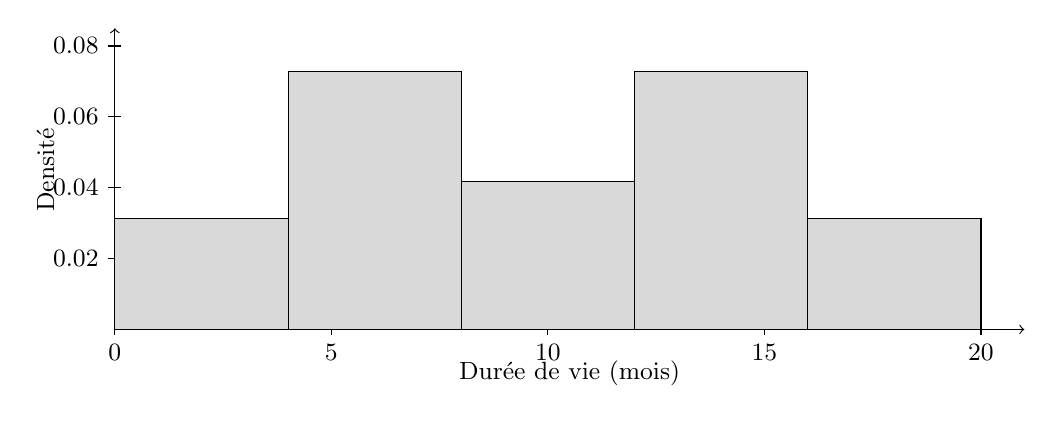
\begin{tikzpicture}[x=0.55cm,y=45cm]
    \draw[->] (0,0) -- (21,0);
    \draw[->] (0,0) -- (0,0.085);
    \foreach \x in {0,5,10,15,20} \draw (\x,0.0015) -- (\x,-0.0015) node[below] {\small \x};
    \foreach \y in {0.02,0.04,0.06,0.08}
      \draw (0.15,\y) -- (-0.15,\y) node[left] {\small \y};
    \filldraw[fill=gray!30] (0,0) rectangle (4,0.03125);
    \filldraw[fill=gray!30] (4,0) rectangle (8,0.0729);
    \filldraw[fill=gray!30] (8,0) rectangle (12,0.0417);
    \filldraw[fill=gray!30] (12,0) rectangle (16,0.0729);
    \filldraw[fill=gray!30] (16,0) rectangle (20,0.03125);
    \node[below] at (10.5,-0.006) {\small Durée de vie (mois)};
    \node[rotate=90] at (-1.6,0.045) {\small Densité};
  \end{tikzpicture}
  \end{center}
  \item Le diagramme en boîte est symétrique, l'histogramme aussi. Or, l'histogramme n'est
  pas \emph{unimodal} (il a deux modes), ce qui implique que la loi normale n'est pas un
  modèle idéal pour ces durées de vie.
\end{enumerate}
\end{solution}
\end{exercice}

\begin{exercice}
Déterminez si les énoncés suivants sont vrais ou faux.
\begin{enumerate}[label=(\alph*)]
  \item Si l'écart-type d'un échantillon est nul, c'est que toutes les observations valent 0.
  \item L'écart-type, la variance et la covariance sont des mesures permettant d'évaluer la
  dispersion des valeurs dans une distribution.
  \item Les valeurs minimale et maximale d'un jeu de données peuvent toujours être
  identifiées sur un diagramme en boîte.
\end{enumerate}
\begin{solution}
\begin{enumerate}[label=(\alph*)]
  \item \textbf{Faux.} Cela signifie que toutes les observations sont \emph{égales} (pas
  nécessairement nulles).
  \item \textbf{Faux.} La covariance n'est pas une mesure de dispersion : elle mesure
  l'association linéaire entre deux variables.
  \item \textbf{Vrai.} Les extrémités des moustaches ou les points au-delà de celles-ci
  permettent toujours de repérer le minimum et le maximum.
\end{enumerate}
\end{solution}
\end{exercice}

\chapitre{6}{Loi échantillonnale et estimation ponctuelle}


\chapitre{7}{Intervalles de confiance}

\begin{exercice}\label{exo:abc}
Vous recueillez 10 échantillons de l'eau rejetée par votre usine ABC. Soit
$x_{ABC,1},\dots,x_{ABC,10}$, les concentrations en plomb (en ppm) de ces échantillons. On
vous dit que leur moyenne échantillonnale est 1,5~ppm et que leur variance échantillonnale
est 0,25~ppm$^2$. On suppose que ces échantillons sont indépendants et identiquement
distribués de loi normale de moyenne et de variance inconnues.

Donnez un intervalle de confiance à 99\,\% pour la concentration moyenne de l'eau rejetée
par l'usine ABC.
\begin{solution}
On a $X_{ABC}\sim N(\mu_{ABC},\sigma^2_{ABC})$, de paramètres inconnus, avec
$\bar x_{ABC}=1,5$~ppm, $s^2_{ABC}=0,25$~ppm$^2$ et $n_{ABC}=10$.
L'intervalle de confiance à 99\,\% pour $\mu_{ABC}$ est
\[
  \bar x_{ABC}\pm t_{\alpha/2;n-1}\frac{s}{\sqrt n}
  =1,5\pm t_{0,005;9}\frac{\sqrt{0,25}}{\sqrt{10}}
  =1,5\pm 3,25(0,158)=1,5\pm 0,51
  =[0,99\,;\;2,01].
\]
\end{solution}
\end{exercice}

\begin{exercice}\label{exo:boites}
À la réception de colis, un responsable doute de l'exactitude des masses affichées sur les
boîtes. Il prélève 25 boîtes au hasard, les pèse et soumet ses résultats à Rcmdr qui produit
la sortie ci-dessous. On supposera que les masses des boîtes suivent une loi normale.
\begin{center}
  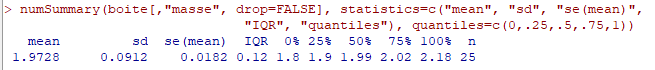
\includegraphics[width=0.95\textwidth]{fig/rcmdr_numsummary}\\[4pt]
  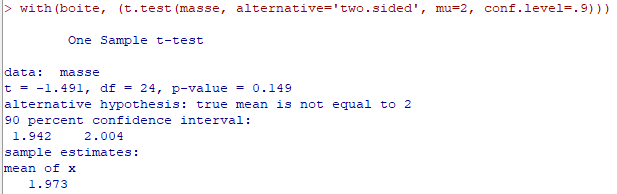
\includegraphics[width=0.75\textwidth]{fig/rcmdr_ttest}
\end{center}
\begin{enumerate}[label=(\alph*)]
  \item Quelle est la marge d'erreur associée à l'estimation de la masse moyenne, pour un
  niveau de confiance de 90\,\% ?
  \item Pour quel niveau de confiance a-t-on un intervalle de confiance pour l'écart-type
  des masses des boîtes de $[0,0712\,;\;0,1269]$ ?
\end{enumerate}
\begin{solution}
\begin{enumerate}[label=(\alph*)]
  \item La marge d'erreur est la demi-longueur de l'intervalle de confiance. C'est aussi la
  différence entre une borne de l'intervalle et la moyenne échantillonnale :
  \[
    \text{marge d'erreur}=2,004-1,973=0,031.
  \]
  On aurait pu la calculer directement à partir de la formule :
  \[
    \text{marge d'erreur}=t_{0,05;24}\frac{s}{\sqrt n}=1,711\times\frac{0,0912}{5}=0,031.
  \]
  \item L'intervalle de confiance de niveau $1-\alpha$ pour un écart-type se calcule avec la
  formule
  \[
    \left[\sqrt{\frac{(n-1)S^2}{\chi^2_{\alpha/2;24}}}\,,\;
    \sqrt{\frac{(n-1)S^2}{\chi^2_{1-\alpha/2;24}}}\right].
  \]
  Prenons la borne inférieure de l'intervalle :
  \[
    \sqrt{\frac{(n-1)s^2}{\chi^2_{\alpha/2;24}}}=0,0712
    \;\Longrightarrow\;
    \chi^2_{\alpha/2;24}=\frac{24\times 0,0912^2}{0,0712^2}=39,38
    \;\Longleftrightarrow\;\alpha/2=0,025\;\Longleftrightarrow\;1-\alpha=0,95.
  \]
\end{enumerate}
\end{solution}
\end{exercice}

\begin{exercice}\label{exo:essieux}
La manufacture pour laquelle vous travaillez produit des essieux. La chaîne de production A
produit présentement des essieux pour votre client qui exige que la variance du diamètre des
essieux ne dépasse pas 1~mm$^2$. Votre client vient vous voir en se plaignant d'une trop
grande variabilité dans le diamètre des derniers essieux livrés. Vous allez avec le client et
sélectionnez 15 essieux au hasard à la sortie de la chaîne de production A. Vous mesurez les
diamètres de ces essieux, que l'on suppose indépendants et distribués selon une loi normale
de moyenne et de variance inconnues, et obtenez une variance échantillonnale de 1,75~mm$^2$.

Donnez un intervalle de confiance à 95\,\% pour la variance du diamètre des essieux produits.
\begin{solution}
L'IC pour $\sigma^2$ est donné par
\[
  \left[\frac{(n-1)S^2}{\chi^2_{\alpha/2;n-1}}\,,\;
  \frac{(n-1)S^2}{\chi^2_{1-\alpha/2;n-1}}\right].
\]
On a $n=15$, $s^2=1,75$ et $\alpha=0,05$. Ainsi,
$\chi^2_{0,025;14}=26,12$ et $\chi^2_{0,975;14}=5,63$, et l'intervalle de confiance pour
$\sigma^2$ est
\[
  \left[\frac{(14)(1,75)}{26,12}\,,\;\frac{(14)(1,75)}{5,63}\right]=[0,94\,;\;4,35].
\]
\end{solution}
\end{exercice}

\begin{exercice}
Déterminez si les énoncés suivants sont vrais ou faux.
\begin{enumerate}[label=(\alph*)]
  \item Lors d'une estimation par intervalle de confiance, les limites de l'intervalle sont
  des constantes de la population.
  \item Dans une loi de Student, la médiane théorique est toujours inférieure à la moyenne
  théorique.
  \item Une compagnie de transport a fait calculer un intervalle de confiance à 95\,\% pour
  le nombre moyen de kilomètres parcourus par ses véhicules en une semaine et a obtenu
  $[62\,050\,;\;74\,110]$. On peut dire qu'il y a 95\,\% de chances que les véhicules de la
  compagnie parcourent entre 62~050 et 74~110~km la semaine prochaine.
\end{enumerate}
\begin{solution}
\begin{enumerate}[label=(\alph*)]
  \item \textbf{Faux.} Les limites de l'intervalle sont des statistiques calculées à partir
  de l'échantillon.
  \item \textbf{Faux.} La loi de Student est symétrique autour de 0 : la médiane théorique
  est toujours égale à la moyenne théorique.
  \item \textbf{Faux.} L'intervalle est construit pour le nombre moyen $\mu$ : la moyenne de
  toutes les valeurs hebdomadaires, et non pour le nombre de km parcourus en une seule
  semaine.
\end{enumerate}
\end{solution}
\end{exercice}

\chapitre{8.1}{Tests d'hypothèses : un échantillon}

\begin{exercice}
On reprend le contexte de l'exercice~\ref{exo:boites} (masses de 25 boîtes,
sortie Rcmdr reproduite ci-dessous).
\begin{center}
  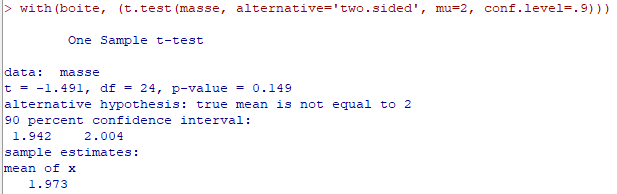
\includegraphics[width=0.75\textwidth]{fig/rcmdr_ttest}
\end{center}
\begin{enumerate}[label=(\alph*)]
  \item Sachant que la masse affichée sur chaque boîte est de 2~kg, les doutes du responsable
  sont-ils justifiés, au seuil de 10\,\% ?
  \item Comment le seuil observé du test ci-dessus a-t-il été calculé ? Écrivez précisément
  la probabilité en question.
\end{enumerate}
\begin{solution}
\begin{enumerate}[label=(\alph*)]
  \item On veut tester
  \[
    H_0:\mu=2\qquad\text{contre}\qquad H_1:\mu\neq 2.
  \]
  Comme dans tous les tests d'hypothèses, on rejette $H_0$ si le seuil observé est inférieur
  à $\alpha$. On retrouve le seuil observé dans la sortie R sous l'appellation
  \texttt{p-value}. (On sait que le test est bilatéral à cause de la commande
  \texttt{two.sided}, et on voit dans la sortie que l'alternative $H_1$ est énoncée comme
  \texttt{true mean is not equal to 2}.) Ici, la valeur $P$ vaut 0,149, supérieure à 10\,\%,
  donc $H_0$ n'est pas rejetée et la masse moyenne ne diffère pas de manière significative
  de 2~kg.
  \item Le seuil observé, c'est-à-dire la valeur de $P$, est la probabilité d'obtenir une
  valeur au moins aussi extrême que celle observée, si on recommençait l'expérience et que
  $H_0$ était vraie :
  \[
    \alpha^*=P(|T|>|t_{obs}|)=P(|T|>1,491)=2\times P(T>1,491)=0,149,
  \]
  où la statistique du test $T$ suit une distribution de Student à 24 degrés de liberté sous
  $H_0$.
\end{enumerate}
\end{solution}
\end{exercice}

\begin{exercice}
Un chercheur s'intéresse à la moyenne $\mu$ d'une certaine variable $X$ distribuée suivant
une loi normale de variance 4. Il veut tester les hypothèses suivantes :
\[
  H_0:\mu=5\qquad\text{contre}\qquad H_1:\mu>5.
\]
Il a prélevé un échantillon aléatoire de taille $n=16$ et a obtenu une moyenne égale à 6,2.
\begin{enumerate}[label=(\alph*)]
  \item La statistique de test et sa loi sous $H_0$ sont
  \[
    \square\ \frac{\bar X-5}{\sigma/\sqrt n}\sim N(0,1)\qquad
    \square\ \frac{\bar X-5}{\sigma/\sqrt n}\sim t_{n-1}\qquad
    \square\ \frac{\bar X-5}{S/\sqrt n}\sim N(0,1)\qquad
    \square\ \frac{\bar X-5}{S/\sqrt n}\sim t_{n-1}
  \]
  \item Dans la figure ci-dessous, identifiez la valeur critique de la moyenne
  échantillonnale au seuil $\alpha=10\,\%$ et hachurez la surface correspondant à ce seuil.
  \begin{center}
    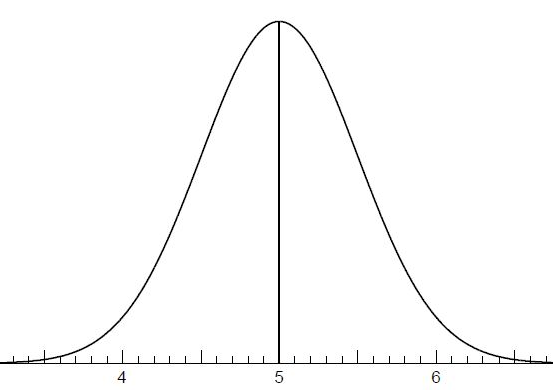
\includegraphics[width=0.55\textwidth]{fig/q_normale_h0}
  \end{center}
  \item Évaluez la valeur $P$ (seuil observé) et hachurez la zone correspondante sur la
  figure ci-dessus.
  \item Supposons qu'en réalité, la vraie moyenne est égale à 6,5. Hachurez la zone associée
  à la puissance du test dans la figure ci-dessous.
  \begin{center}
    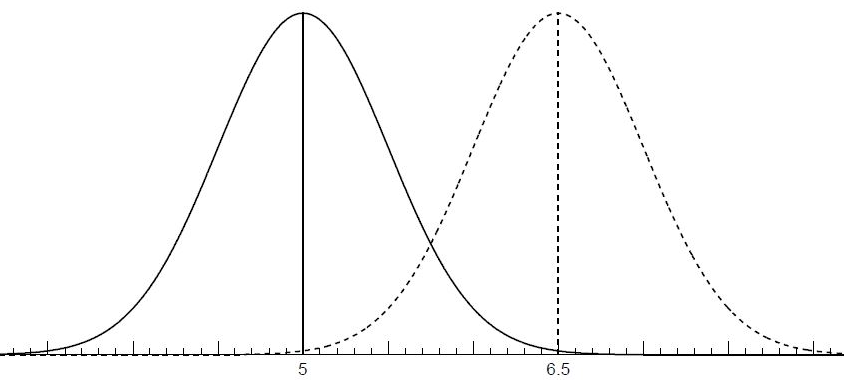
\includegraphics[width=0.7\textwidth]{fig/q_normale_h0h1}
  \end{center}
\end{enumerate}
\begin{solution}
\begin{enumerate}[label=(\alph*)]
  \item Comme la variance est \emph{connue} ($\sigma^2=4$), la statistique de test est
  \[
    \blacksquare\ \frac{\bar X-5}{\sigma/\sqrt n}\sim N(0,1).
  \]
  \item On rejette $H_0$ si $\frac{\bar X-5}{2/\sqrt{16}}>z_{0,10}=1,28$, donc si
  $\bar x>(1,28)(2/4)+5=5,64$.
  \begin{center}
    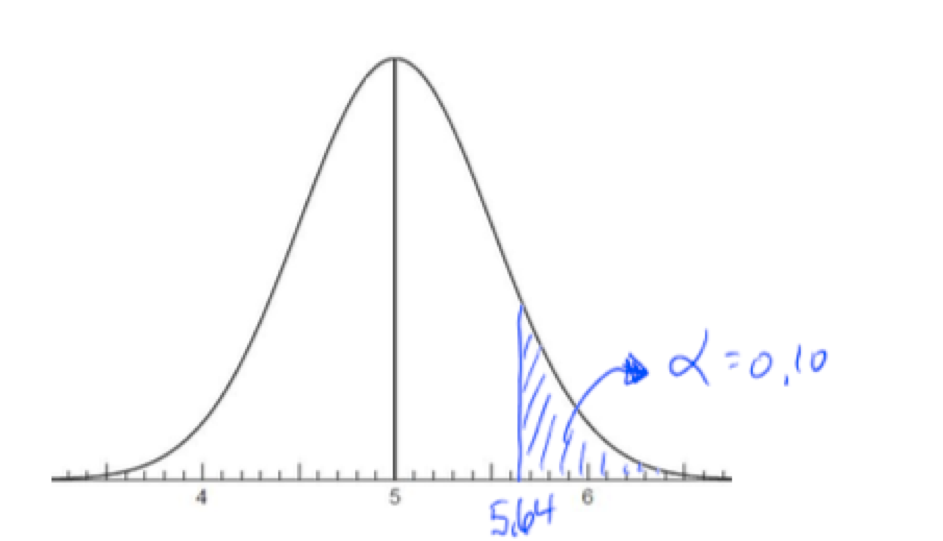
\includegraphics[width=0.6\textwidth]{fig/sol_q6b}
  \end{center}
  \item
  \[
    \alpha^*=P(\bar X>6,2)=P\!\left(Z>\frac{6,2-5}{2/4}\right)=P(Z>2,4)=0,0082.
  \]
  La zone hachurée correspondante (sous $H_0$, à droite de 6,2) est illustrée ci-dessous
  (en vert).
  \begin{center}
    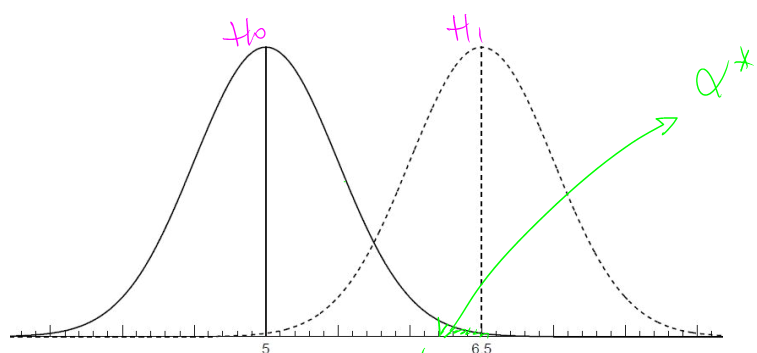
\includegraphics[width=0.7\textwidth]{fig/sol_q6c}
  \end{center}
  \item La zone associée à la puissance est la surface sous la courbe de $H_1$ (centrée à
  6,5) à droite de la valeur critique 5,64 (en rouge sur la figure ci-dessous). Le calcul
  exact n'était pas demandé, mais on aurait pu l'obtenir comme suit :
  \[
    1-\beta=P(\text{Rejeter }H_0\,|\,H_1\text{ vraie})
    =P(\bar X>5,64\,|\,\mu=6,5)
    =P\!\left(Z>\frac{5,64-6,5}{2/4}\right)=P(Z>-1,72)=0,9573.
  \]
  \begin{center}
    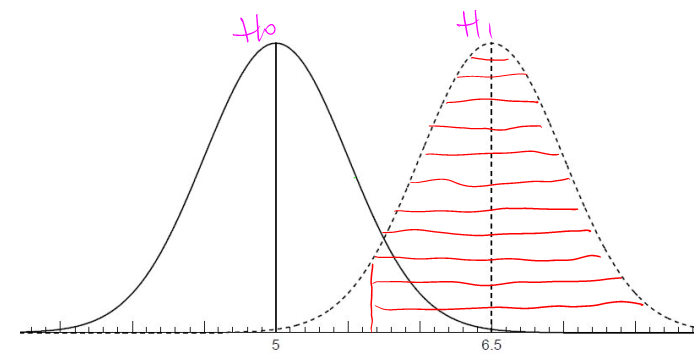
\includegraphics[width=0.7\textwidth]{fig/sol_q6d}
  \end{center}
\end{enumerate}
\end{solution}
\end{exercice}

\begin{exercice}
On reprend le contexte de l'exercice~\ref{exo:essieux} (diamètres de 15
essieux, $s^2=1,75$~mm$^2$; le client exige que la variance ne dépasse pas 1~mm$^2$).
\begin{enumerate}[label=(\alph*)]
  \item Y a-t-il de l'évidence au seuil de 5\,\% que le client a raison et que la variance
  excède 1~mm$^2$ ?
  \item Quel est le plus petit seuil à partir duquel on peut rejeter l'hypothèse nulle
  en~(a) ?
  \item Que vaut la probabilité d'erreur de type II si la vraie variance des diamètres est
  de 2~mm$^2$ ?
\end{enumerate}
\begin{solution}
\begin{enumerate}[label=(\alph*)]
  \item On veut tester $H_0:\sigma^2=1$ contre $H_1:\sigma^2>1$ au seuil de 5\,\%.
  On rejette $H_0$ si $U_0>\chi^2_{\alpha;n-1}=\chi^2_{0,05;14}=23,68$.
  La valeur observée de la statistique du test est
  \[
    u_0=\frac{(n-1)s^2}{\sigma_0^2}=\frac{(15-1)(1,75)}{1}=24,5.
  \]
  Comme $u_0>23,68$, on rejette $H_0$ et on conclut que oui, le client a raison et la
  variance est significativement supérieure à 1.
  \item La statistique du test est $U=\frac{(n-1)S^2}{\sigma_0^2}$ qui suit une loi
  $\chi^2_{14}$ sous $H_0$ :
  \[
    \alpha^*=P(U>24,5)\in[0,025\,;\;0,05]\text{ selon la table.}
  \]
  \begin{center}
    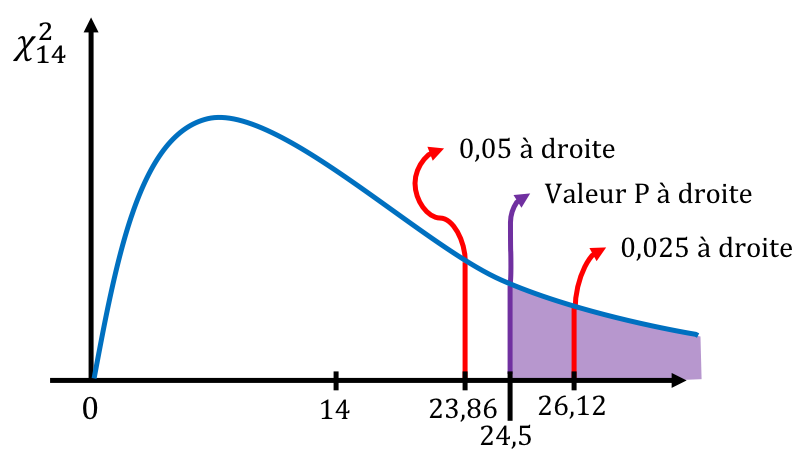
\includegraphics[width=0.6\textwidth]{fig/sol_chi2}
  \end{center}
  \item Notons que $(n-1)\frac{S^2}{1}\sim\chi^2_{14}$ si $H_0:\sigma^2=1$ est vraie, et que
  $(n-1)\frac{S^2}{2}\sim\chi^2_{14}$ si $H_1:\sigma^2=2$ est vraie. Alors
  \begin{align*}
    \beta&=P(\text{ne pas rejeter }H_0\,|\,H_1\text{ est vraie})
    =P\!\left((n-1)\tfrac{S^2}{1}<23,68\,\Big|\,\sigma^2=2\right)\\
    &=P\!\left((n-1)\tfrac{S^2}{2}<\tfrac{23,68}{2}\right)
    =P(U_1<11,84)\in[0,10\,;\;0,50]
  \end{align*}
  selon la table des quantiles d'une $\chi^2$ à 14 degrés de liberté. Avec un logiciel, on
  trouve 0,38.
\end{enumerate}
\end{solution}
\end{exercice}

\begin{exercice}
Déterminez si les énoncés suivants sont vrais ou faux.
\begin{enumerate}[label=(\alph*)]
  \item Lors d'un test d'hypothèses, plus le seuil observé est faible, plus notre
  échantillon semble plausible sous $H_0$.
  \item La puissance d'un test d'hypothèses augmente lorsqu'on augmente la taille de
  l'échantillon (si rien d'autre ne change).
  \item Dans un test d'hypothèses, on rejette toujours l'hypothèse nulle si le seuil observé
  (p-value) est plus grand que le seuil du test.
  \item On teste l'hypothèse $H_0:\sigma^2=4$ contre $H_1:\sigma^2\neq 4$ et on obtient un
  seuil observé de 0,1433. On peut dire que l'intervalle de confiance à 90\,\% pour la
  variance ne contient pas la valeur 4.
  \item On construit un intervalle de confiance à 95\,\% pour la durée moyenne (en minutes)
  d'un appel au service à la clientèle et on obtient : $[6,3\,;\;8,1]$. On peut dire qu'au
  seuil de 5\,\%, on rejette l'hypothèse que $\mu=6$, au profit de l'hypothèse alternative
  $\mu\neq 6$.
\end{enumerate}
\begin{solution}
\begin{enumerate}[label=(\alph*)]
  \item \textbf{Faux.} Plus le seuil observé est faible, plus notre échantillon semble
  \emph{extrême} sous $H_0$.
  \item \textbf{Vrai.}
  \item \textbf{Faux.} On rejette l'hypothèse nulle si le seuil observé est plus
  \emph{petit} que le seuil du test.
  \item \textbf{Faux.} $H_0$ n'est pas rejetée, car le seuil observé est supérieur à
  10\,\%. Ainsi, $4\in IC(\sigma^2)$ à 90\,\%.
  \item \textbf{Vrai.}
\end{enumerate}
\end{solution}
\end{exercice}

\chapitre{8.2}{Tests d'hypothèses : deux échantillons}

\begin{exercice}
On reprend le contexte de l'exercice~\ref{exo:abc} (10 échantillons d'eau de
l'usine ABC : $\bar x_{ABC}=1,5$~ppm, $s^2_{ABC}=0,25$~ppm$^2$).
\begin{enumerate}[label=(\alph*)]
  \item Vous recueillez 10 échantillons d'eau de votre usine XYZ, disons
  $x_{XYZ,1},\dots,x_{XYZ,10}$, dont la moyenne échantillonnale est 1,6~ppm et la variance
  échantillonnale est 0,22~ppm$^2$. On suppose aussi que ces échantillons proviennent d'une
  population normale de moyenne et de variance inconnues. Testez, au seuil de 5\,\%, si les
  variances des concentrations échantillonnées dans l'eau rejetée par les deux usines sont
  égales.
  \item En supposant les variances égales, a-t-on suffisamment d'évidence, au seuil de
  5\,\%, pour dire que la concentration en plomb dans l'eau rejetée par l'usine ABC est
  inférieure à celle de l'eau rejetée par l'usine XYZ en moyenne ?
\end{enumerate}
\begin{solution}
\begin{enumerate}[label=(\alph*)]
  \item On a $X_{XYZ}\sim N(\mu_{XYZ},\sigma^2_{XYZ})$, de paramètres inconnus, avec
  $\bar x_{XYZ}=1,6$~ppm, $s^2_{XYZ}=0,22$~ppm$^2$ et $n_{XYZ}=10$. On teste
  \[
    H_0:\sigma^2_{ABC}=\sigma^2_{XYZ}\qquad\text{contre}\qquad
    H_1:\sigma^2_{ABC}\neq\sigma^2_{XYZ}.
  \]
  \emph{Règle de décision :} on rejette $H_0$ si
  $f_0<F_{1-\alpha/2;9;9}=\frac{1}{F_{0,025;9,9}}=\frac{1}{4,03}=0,248$ ou si
  $f_0>F_{0,025;9,9}=4,03$.

  \emph{Calcul de la valeur observée de la statistique :}
  \[
    f_0=\frac{s^2_{ABC}}{s^2_{XYZ}}=\frac{0,25}{0,22}=1,136.
  \]
  \emph{Décision :} puisque 1,136 n'est ni supérieur à 4,03 ni inférieur à 0,248, on ne
  rejette pas $H_0$.

  \emph{Conclusion :} les variances des concentrations de plomb aux deux usines ne diffèrent
  pas de façon significative au seuil de 5\,\%.
  \item On peut utiliser le test de Student pour deux échantillons indépendants avec
  variances théoriques égales. On estimera donc $\sigma^2_{ABC}=\sigma^2_{XYZ}=\sigma^2$
  par une mesure commune combinant les deux variances échantillonnales. On teste
  \[
    H_0:\mu_{ABC}=\mu_{XYZ}\qquad\text{contre}\qquad H_1:\mu_{ABC}<\mu_{XYZ}.
  \]
  \emph{Règle de décision :} on rejette $H_0$ si
  $t_0<-t_{0,05;18}=-1,734$.

  \emph{Calcul de la valeur observée de la statistique :}
  \[
    s_p=\sqrt{\frac{(n_{ABC}-1)s^2_{ABC}+(n_{XYZ}-1)s^2_{XYZ}}{n_{ABC}+n_{XYZ}-2}}
    =\sqrt{\frac{9(0,25)+9(0,22)}{18}}=\sqrt{0,235}=0,485,
  \]
  \[
    t_0=\frac{\bar x_{ABC}-\bar x_{XYZ}}{s_p\sqrt{\frac{1}{10}+\frac{1}{10}}}
    =\frac{1,5-1,6}{0,485\sqrt{0,2}}=-0,46.
  \]
  \emph{Décision :} puisque $-0,46$ n'est pas inférieur à $-1,734$, on ne rejette pas $H_0$.

  \emph{Conclusion :} la concentration moyenne de plomb à l'usine ABC n'est pas
  significativement inférieure à celle de l'usine XYZ au seuil de 5\,\%.
\end{enumerate}
\end{solution}
\end{exercice}

\begin{exercice}
Nous avons mesuré des arbres debout par une méthode trigonométrique. Pour vérifier la
fiabilité de la méthode, les mêmes arbres ont été à nouveau mesurés, mais au sol après
abattage. Les tailles en mètres pour six arbres et pour les deux méthodes de mesure sont
données dans le tableau suivant :
\begin{center}
\begin{tabular}{lcccccc}
  \toprule
  Arbre & 1 & 2 & 3 & 4 & 5 & 6\\
  \midrule
  Debout & 20 & 25 & 25 & 25 & 26 & 28\\
  Abattu & 21 & 26 & 26 & 28 & 26 & 27\\
  \bottomrule
\end{tabular}
\end{center}
On admet que la variable étudiée est normalement distribuée.
\begin{enumerate}[label=(\alph*)]
  \item Ces résultats permettent-ils de dire, au niveau de signification $\alpha=0,01$, que
  la méthode trigonométrique sous-estime les longueurs des arbres par rapport à la mesure
  des arbres abattus ?
  \item Quel est le seuil observé du test ?
\end{enumerate}
\begin{solution}
\begin{enumerate}[label=(\alph*)]
  \item On veut tester les hypothèses suivantes :
  \[
    H_0:\mu_{debout}=\mu_{abattu}\qquad\text{contre}\qquad
    H_1:\mu_{debout}<\mu_{abattu},
  \]
  avec $\alpha=0,01$. On a 6 arbres sur lesquels on a pris 2 mesures (et non 12 arbres sur
  lesquels on a pris des mesures indépendantes). Il faut donc utiliser le test pour
  \emph{données appariées}. On utilisera les 6 différences
  $\{d_1,\dots,d_6\}=\{-1,-1,-1,-3,0,1\}$ et le test s'appliquera à un échantillon de
  différences. Les hypothèses deviennent $H_0:\mu_D=0$ contre $H_1:\mu_D<0$, avec
  $\mu_D=\mu_{debout}-\mu_{abattu}$.

  \emph{Règle de décision :} on rejettera $H_0$ si
  $T_0=\frac{\bar D}{S_D/\sqrt n}<-t_{0,01;5}=-3,365$.

  \emph{Statistique du test et calcul de sa valeur :} avec $\bar d=-\frac56$ et
  $s_D=\sqrt{\frac{\sum_{i=1}^{6}(d_i-\bar d)^2}{n-1}}=1,329$,
  \[
    t_0=\frac{-5/6}{1,329/\sqrt 6}=-1,536.
  \]
  \emph{Décision :} comme $-1,536\not<-3,365$, on ne rejette pas $H_0$.

  \emph{Conclusion :} la méthode trigonométrique ne sous-estime pas la longueur de façon
  significative au seuil de 1\,\%.
  \begin{center}
    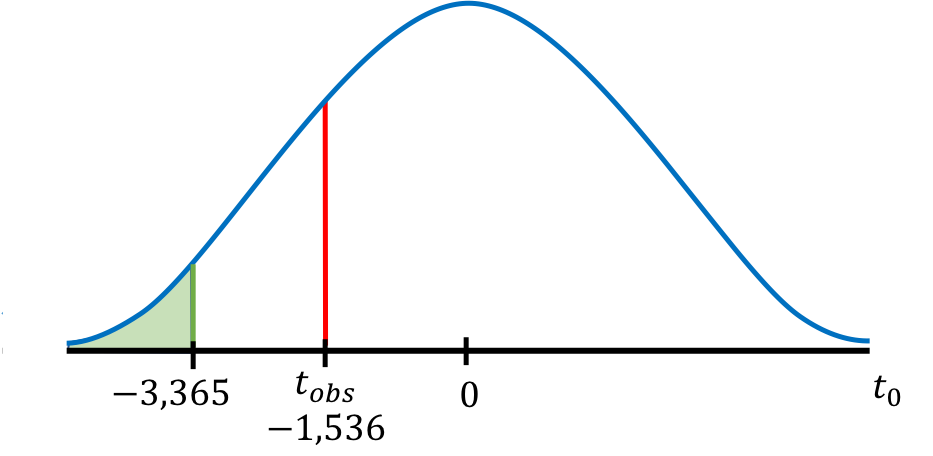
\includegraphics[width=0.55\textwidth]{fig/sol_arbres1}
  \end{center}
  \item Le seuil observé est la valeur-$p$, notée $\alpha^*$ : la probabilité d'obtenir une
  valeur au moins aussi extrême (ici, aussi petite) que celle observée, si $H_0$ était
  vraie. C'est aussi le plus petit seuil permettant de rejeter $H_0$ avec les valeurs
  observées :
  \[
    \alpha^*=P(T<-1,536)\in[0,05\,;\;0,10]
  \]
  selon la table des quantiles de Student avec 5 degrés de liberté. Avec un logiciel, on
  trouve que $\alpha^*=0,093$.
  \begin{center}
    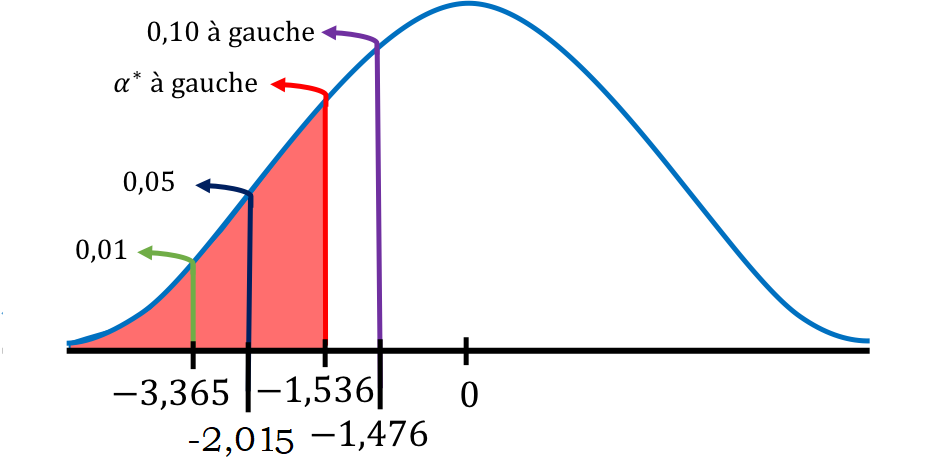
\includegraphics[width=0.55\textwidth]{fig/sol_arbres2}
  \end{center}
\end{enumerate}
\end{solution}
\end{exercice}

\begin{exercice}
Vous voulez recruter dans votre équipe le golfeur dont la longueur des coups de départ est
la moins variable entre Tiger et Rory. Vous pensez qu'il s'agit de Tiger mais pour être
certain vous les mettez à l'essai : Tiger frappe 9 coups de départ alors que Rory en frappe
7. L'écart-type échantillonnal de la longueur des coups de départ frappés par Tiger est de 8
verges alors que l'écart-type échantillonnal des coups de départ frappés par Rory est de 10
verges. Au seuil de 5\,\%, peut-on conclure que les coups de départ de Tiger sont moins
variables que ceux de Rory ?
\begin{solution}
On teste
\[
  H_0:\sigma^2_T=\sigma^2_R\qquad\text{contre}\qquad H_1:\sigma^2_T<\sigma^2_R.
\]
\emph{Règle de décision :} on rejette $H_0$ si
\[
  F_0=\frac{S^2_T}{S^2_R}<F_{0,95;8,6}=\frac{1}{F_{0,05;6,8}}=\frac{1}{3,58}=0,279.
\]
\emph{Statistique du test et calcul de sa valeur :}
\[
  f_{obs}=\frac{s^2_T}{s^2_R}=\frac{8^2}{10^2}=0,64.
\]
\emph{Décision :} puisque $f_{obs}>0,279$, on ne rejette pas $H_0$.

\emph{Conclusion :} au seuil de 5\,\%, la longueur des coups de Tiger n'est pas moins
variable que celle des coups de Rory.
\end{solution}
\end{exercice}

\begin{exercice}
Pour la conception de nouveaux circuits électriques, on souhaite comparer les résistances de
deux types de composants électriques. On prend alors un échantillon de composants de chaque
type et on teste leurs résistances (en ohms, notés $\Omega$). Voici un résumé de la collecte
de données.
\begin{center}
\begin{tabular}{lccc}
  \toprule
  Échantillons & Taille & Moyenne & Écart-type\\
  \midrule
  Type 1 & 10 & $404,6\ \Omega$ & $9,23\ \Omega$\\
  Type 2 & 10 & $395,2\ \Omega$ & $6,07\ \Omega$\\
  \bottomrule
\end{tabular}
\end{center}
On a soumis les données aux commandes de la fenêtre de gauche ci-dessous, puis on a obtenu
les résultats présentés dans la fenêtre de droite.
\begin{center}
  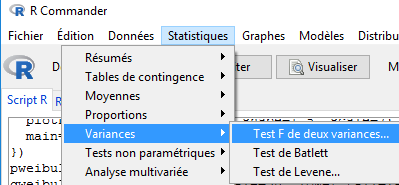
\includegraphics[width=0.48\textwidth]{fig/rcmdr_menu_var}\hfill
  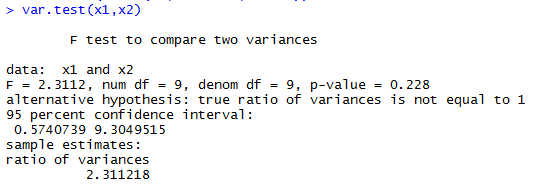
\includegraphics[width=0.48\textwidth]{fig/rcmdr_vartest}
\end{center}
On considère que la loi normale est un modèle acceptable pour la résistance des composants.
On choisit de faire toutes les analyses au seuil de 10\,\%.
\begin{enumerate}[label=(\alph*)]
  \item Pour comparer statistiquement les résistances \emph{moyennes} des composants de type
  1 et de type 2, lequel des tests suivants serait le plus adéquat ? Pourquoi ?
  \begin{itemize}
    \item[$\square$] Le test de Student pour des données appariées ($t_{n-1}$)
    \item[$\square$] Le test de Student pour échantillons indépendants, où on considère que
    $\sigma^2_1=\sigma^2_2$ ($t_{n_1+n_2-2}$)
    \item[$\square$] Le test de Welch pour échantillons indépendants, où on considère que
    $\sigma^2_1\neq\sigma^2_2$ ($t^*_v$)
    \item[$\square$] Le test de Fisher pour échantillons indépendants ($F_{n_1-1,n_2-1}$)
  \end{itemize}
  Justifiez votre choix, en précisant les valeurs numériques que vous interprétez (s'il y a
  lieu).
  \item Au seuil de 10\,\%, peut-on dire que la résistance des composants de type 1 diffère
  de celle des composants de type 2 en moyenne ? Répondre à la question en détaillant toutes
  les étapes d'un test d'hypothèses.

  \emph{Raccourcis de calculs selon le type d'analyse que vous avez choisi :}
  \begin{itemize}
    \item Données appariées : utilisez la variance $s^2_D=9,51^2$
    \item Test de Student : utilisez la variance $s^2_p=7,81^2$
    \item Test de Welch : utilisez les degrés de liberté $v=16$
  \end{itemize}
  \item Quelle est la valeur $P$ (seuil observé) du test réalisé à la question précédente ?
  (Donnez un intervalle de valeurs le plus précis possible en fonction des tables de lois
  dont vous disposez. Écrivez clairement la probabilité calculée, ainsi que sa valeur.)
\end{enumerate}
\begin{solution}
\begin{enumerate}[label=(\alph*)]
  \item $\blacksquare$ Le test de Student pour échantillons indépendants, où on considère
  que $\sigma^2_1=\sigma^2_2$ ($t_{n_1+n_2-2}$).

  Le seuil observé du test de comparaison des variances vaut 0,228, supérieur à 10\,\%,
  donc les variances ne diffèrent pas de façon significative. On peut donc utiliser le test
  de Student avec variances égales. De plus, les échantillons sont collectés de manière
  indépendante, rien n'indique qu'ils sont appariés.
  \item On veut tester
  \[
    H_0:\mu_1=\mu_2\qquad\text{contre}\qquad H_1:\mu_1\neq\mu_2.
  \]
  \emph{Règle de décision :} on rejettera $H_0$ si
  \[
    |t_0|=\left|\frac{\bar X_1-\bar X_2}{S_p\sqrt{\frac{1}{n_1}+\frac{1}{n_2}}}\right|
    >t_{0,05;18}=1,734.
  \]
  \emph{Statistique du test et calcul de sa valeur :} l'estimation globale de la variance
  est donnée, mais elle se calculerait comme suit :
  \[
    s^2_p=\frac{(10-1)(9,23)^2+(10-1)(6,07)^2}{10+10-2}=61,02=(7,81)^2.
  \]
  La valeur observée de la statistique du test est
  \[
    t_0=\frac{404,6-395,2}{7,81\sqrt{\frac{1}{10}+\frac{1}{10}}}=2,691.
  \]
  \emph{Décision :} puisque $|t_0|$ est supérieur à 1,734, nous rejetons $H_0$.

  \emph{Conclusion :} les résistances moyennes diffèrent de manière significative au seuil
  de 10\,\%.
  \item Le seuil observé est la probabilité d'obtenir une valeur au moins aussi extrême que
  celle observée, si on recommençait l'expérience et que $H_0$ était vraie. Considérons
  $T\sim t_{18}$ :
  \[
    \alpha^*=P(|T|>|t_{obs}|)=P(|T|>2,69)=2\times P(T>2,69)=0,02.
  \]
\end{enumerate}
\end{solution}
\end{exercice}

\begin{exercice}
Déterminez si l'énoncé suivant est vrai ou faux.
\begin{enumerate}[label=(\alph*)]
  \item Il est avantageux d'utiliser l'appariement dans une expérience quand les unités
  expérimentales sont homogènes.
\end{enumerate}
\begin{solution}
\begin{enumerate}[label=(\alph*)]
  \item \textbf{Faux.} Il est avantageux d'utiliser l'appariement dans une expérience quand
  les unités expérimentales sont \emph{hétérogènes}.
\end{enumerate}
\end{solution}
\end{exercice}

\chapitre{9}{Analyse de la variance (ANOVA)}

\begin{exercice}
Pour chacune des situations suivantes, choisissez le type d'analyse statistique approprié.
Identifiez les variables (en considérant que toutes les variables spécifiées sont incluses
dans le modèle), et le nombre de degrés de liberté associés à l'erreur.
\begin{enumerate}[label=(\alph*)]
  \item Vous souhaitez comparer la consommation d'essence de 3 modèles de voiture. Vous
  n'êtes pas intéressé par la variation de la consommation d'essence entre les conducteurs,
  mais vous vous attendez à ce que le style de conduite ait un effet important sur la
  consommation d'essence. Vous planifiez une expérience où 5 personnes conduisent (une fois
  chacune) les voitures des trois modèles sur un circuit déterminé, dans un ordre aléatoire.
  Chaque essai est réalisé sur le même parcours dans des conditions de température et d'état
  de la chaussée similaires.
  \item Depuis 24 ans, un cultivateur note le rendement (en kg/hectare) de ses cultures de
  blé, la quantité de pluie reçue chaque mois ainsi que la température moyenne de chaque
  mois. Vous souhaitez utiliser ses données pour construire un modèle qui lui permettra de
  prédire le rendement de ses cultures de blé en fonction de la température moyenne des mois
  de juin et juillet, et de la quantité de pluie reçue en juin et en juillet.
  \item Vous voulez vérifier l'effet de la profondeur du sol et l'effet de la topographie du
  site sur la quantité de phosphore dans le sol. Vous vous attendez à ce que l'effet de la
  profondeur varie selon la topographie, et vous tenez à ce que votre modèle en tienne
  compte. Vous sélectionnez 15 sites où la topographie est plane et 15 sites où la
  topographie est en pente.
  \begin{itemize}
    \item 5 sites planes sont choisis au hasard : sur chacun, vous prendrez un échantillon
    de sol à 5~cm de profondeur et en mesurerez le phosphore ;
    \item 5 autres sites planes sont choisis au hasard : sur chacun, vous prendrez un
    échantillon de sol à 10~cm de profondeur et en mesurerez le phosphore ;
    \item sur les 5 sites planes restants, vous prendrez un échantillon de sol à 20~cm de
    profondeur et en mesurerez le phosphore ;
    \item vous répéterez les 3 étapes ci-dessus pour les 15 sites en pente ;
    \item les 30 mesures de phosphore décrites ci-dessus seront prises dans un ordre
    aléatoire.
  \end{itemize}
  \item Un inspecteur en alimentation se demande si la quantité de pesticides sur les fruits
  et légumes que l'on retrouve sur le marché est associée à la taille des fermes
  maraîchères. En juillet, il visite 15 producteurs de fraises québécois choisis
  aléatoirement. Pour chacun, il analyse la quantité de pesticides dans un panier de
  fraises, et la met en relation avec les ventes de fraises de l'année précédente de ce
  producteur.
\end{enumerate}
\begin{solution}
\begin{enumerate}[label=(\alph*)]
  \item Analyse de la variance avec blocs aléatoires.\\
  Variable réponse : consommation d'essence.\\
  Facteur : modèle de voiture ($a=3$). Bloc : conducteur ($b=5$).\\
  Degrés de liberté à l'erreur : $(a-1)(b-1)=8$.
  \item Régression linéaire multiple.\\
  Variable réponse : rendement des cultures de blé.\\
  Variables explicatives : température en juin, température en juillet, pluie en juin,
  pluie en juillet ($k=4$).\\
  Degrés de liberté à l'erreur : $n-k-1=19$.
  \item Analyse de la variance à deux facteurs.\\
  Variable réponse : quantité de phosphore dans le sol.\\
  Facteurs : topographie ($a=2$), profondeur ($b=3$) [et leur interaction].\\
  Degrés de liberté à l'erreur : $ab(n-1)=24$.
  \item Régression linéaire simple.\\
  Variable réponse : quantité de pesticides sur un panier de fraises.\\
  Variable explicative : ventes de fraises l'année précédente.\\
  Degrés de liberté à l'erreur : $n-2=13$.
\end{enumerate}
\end{solution}
\end{exercice}

\begin{exercice}
Votre manufacture produit des tiges métalliques qui sont utilisées dans la confection de
prothèses. La résistance de ces tiges à la torsion est une propriété très importante. Vous
désirez savoir si le type d'alliage utilisé pour produire les tiges a un effet sur leur
résistance à la torsion. À partir de chacun de trois types d'alliage (1, 2 et 3), vous
produisez quatre tiges et les soumettez à un test de torsion. Soit $Y_{ij}$, la torsion (en
Nm) menant à la rupture de la tige $j$ produite avec l'alliage $i$. Le tableau ci-dessous
vous donne la valeur observée $y_{ij}$ pour chacune des 12 tiges testées.
\begin{center}
\begin{tabular}{c*{4}{c}cc}
  \toprule
  Alliage & \multicolumn{4}{c}{Torsion de rupture (en Nm)} & Somme & Moyenne\\
  $i$ & Tige 1 & Tige 2 & Tige 3 & Tige 4 & $y_{i\bullet}$ & $\bar y_{i\bullet}$\\
  \midrule
  1 & 510 & 490 & 520 & 480 & 2\,000 & 500\\
  2 & 500 & 510 & 540 & 530 & 2\,080 & 520\\
  3 & 500 & 490 & 470 & 460 & 1\,920 & 480\\
  \midrule
  Total & & & & & $y_{\bullet\bullet}=6\,000$ & $\bar y_{\bullet\bullet}=500$\\
  \bottomrule
\end{tabular}
\end{center}
Supposons que le modèle d'analyse de la variance
\[
  (*)\qquad Y_{ij}=\mu+\tau_i+E_{ij},\qquad i=1,\dots,3,\ j=1,\dots,4,
\]
avec les $E_{ij}$ indépendantes de loi $N(0,\sigma^2)$ est un modèle adéquat.
\begin{enumerate}[label=(\alph*)]
  \item Dans le modèle (*) d'analyse de la variance ci-dessus, $\tau_2$ représente
  \begin{itemize}
    \item[$\square$] la torsion de rupture moyenne des tiges produites avec l'alliage 2 ;
    \item[$\square$] la torsion de rupture moyenne de la deuxième tige produite avec les
    trois alliages ;
    \item[$\square$] la différence entre la torsion de rupture moyenne des tiges produites
    avec l'alliage 2 et la torsion de rupture moyenne de l'ensemble des tiges produites avec
    les trois alliages.
  \end{itemize}
  \item Une estimation de la valeur de $\tau_2$ est donnée par :
  \item En plus de l'information du tableau ci-dessus, on vous donne
  \[
    \sum_{i=1}^{3}\sum_{j=1}^{4}y^2_{ij}=3\,006\,200
    \qquad\text{et}\qquad SSE=3\,000.
  \]
  Construisez le tableau d'analyse de la variance. Au seuil de 5\,\%, est-ce que le type
  d'alliage a un effet significatif sur la torsion de rupture ?
  \item Supposons qu'à l'étape précédente, vous avez conclu qu'il existait des différences
  significatives entre les moyennes, en général. Pouvez-vous déterminer au seuil de 5\,\%
  quels alliages précisément diffèrent les uns des autres ?
\end{enumerate}
\begin{solution}
\begin{enumerate}[label=(\alph*)]
  \item $\blacksquare$ la différence entre la torsion de rupture moyenne des tiges produites
  avec l'alliage 2 et la torsion de rupture moyenne de l'ensemble des tiges produites avec
  les trois alliages.
  \item Une estimation de la valeur de $\tau_2$ est donnée par
  \[
    \hat\tau_2=\bar y_{2\bullet}-\bar y_{\bullet\bullet}=520-500=20.
  \]
  \item La somme donnée permet de calculer facilement
  \[
    SST=\sum_i\sum_j y^2_{ij}-y^2_{\bullet\bullet}/ab=3\,006\,200-6000^2/12=6200.
  \]
  On obtient ensuite par soustraction
  $SS_{trt}=SST-SSE=6200-3000=3200$. Notons qu'on aurait aussi pu calculer $SS_{trt}$
  directement comme suit :
  \[
    SS_{trt}=n\sum_{i=1}^{3}\hat\tau_i^2=4\left(0^2+20^2+(-20)^2\right)=3200.
  \]
  Il ne nous reste qu'à compléter le tableau :
  \begin{center}
  \begin{tabular}{lcccc}
    \toprule
    Source de variabilité & Somme des carrés & d.l. & Carré moyen & $F_0$\\
    \midrule
    Traitement & 3200 & $3-1=2$ & $\frac{3200}{2}=1600$ & $\frac{1600}{333,33}=4,8$\\[3pt]
    Erreur & 3000 & $12-3=9$ & $\frac{3000}{9}=333,33$ & \\[3pt]
    Totale & 6200 & $12-1=11$ & & \\
    \bottomrule
  \end{tabular}
  \end{center}
  \emph{Règle de décision :} on rejette $H_0:\mu_1=\mu_2=\mu_3$ si
  $F_0>F_{0,05;2,9}=4,26$.

  \emph{Décision :} puisque $f_{obs}=4,8$ est supérieur à 4,26, alors on rejette $H_0$.

  \emph{Conclusion :} au moins 2 alliages diffèrent de façon significative. Le type
  d'alliage a un effet significatif sur la torsion moyenne.
  \item On peut comparer les moyennes 2 à 2. Celles dont la différence excède la PPDS seront
  déclarées significativement différentes :
  \[
    PPDS=t_{\frac{\alpha}{2};an-a}\sqrt{\frac{MSE}{n}+\frac{MSE}{n}}
    =t_{0,025;9}\sqrt{\frac{2MSE}{4}}=2,262\sqrt{\frac{2(333,33)}{4}}=29,20.
  \]
  On a :
  \begin{center}
  \begin{tabular}{ccc}
    $\bar y_{3\bullet}$ & $\bar y_{1\bullet}$ & $\bar y_{2\bullet}$\\
    480 & 500 & 520\\
  \end{tabular}
  \end{center}
  Les seules moyennes qui diffèrent significativement sont celles des alliages 2 et 3, car
  leurs moyennes diffèrent de 40, ce qui est supérieur à 29,20.
\end{enumerate}
\end{solution}
\end{exercice}

\begin{exercice}
On effectue une expérience afin de déterminer si le type de suspension a un effet sur la
distance de freinage d'un prototype de voiture. Comme la distance de freinage peut varier
beaucoup en fonction de la température et du niveau d'humidité, on décide de mener
l'expérience sur 5 jours différents, toujours avec le même conducteur. À chaque jour, on
testera les 3 types de suspension, une fois chacun, en amenant la voiture à 120~km/h, en
appliquant les freins et en mesurant la distance de freinage.
\begin{enumerate}[label=(\alph*)]
  \item Dites lequel parmi la distance de freinage, le jour, le conducteur et le type de
  suspension correspond au facteur, au bloc et à la variable réponse.
\end{enumerate}
Les questions (b) à (d) portent sur l'extrait de sortie R Commander ci-dessous, qui donne
les résultats d'une analyse de la variance avec blocs aléatoires faite sur les données
décrites ci-dessus.
\begin{verbatim}
Anova Table (Type II tests)
Response: Distance
            Sum Sq    Df   F value    Pr(>F)
Suspension  169.41  AAAAA   DDDDD    0.02418 *
Jour       2338.66  BBBBB   EEEEE  1.984e-05 ***
Residuals   110.31  CCCCC
\end{verbatim}
\begin{enumerate}[label=(\alph*),resume]
  \item Des valeurs ont été effacées dans la sortie et remplacées par AAAAA, BBBBB, etc.
  Trouvez ces valeurs manquantes.
  \item Le type de suspension a-t-il un effet significatif sur la distance de freinage au
  seuil de 1\,\% ?
  \item À la lumière des résultats obtenus, est-ce qu'utiliser une expérience par blocs
  aléatoires était une bonne idée ?
\end{enumerate}
\begin{solution}
\begin{enumerate}[label=(\alph*)]
  \item Facteur : type de suspension. Réponse : distance de freinage. Bloc : jour.
  \item ~
  \begin{align*}
    \text{AAAAA}&=a-1=3-1=2\\
    \text{BBBBB}&=b-1=5-1=4\\
    \text{CCCCC}&=(a-1)(b-1)=8\\
    \text{DDDDD}&=\frac{MSA}{MSE}=\frac{169,41/2}{110,31/8}=6,14\\
    \text{EEEEE}&=\frac{MSB}{MSE}=\frac{2338,66/4}{110,31/8}=42,40
  \end{align*}
  \item $P(F_{2,8}>6,14)=0,02418$ (de la sortie R Commander). Comme
  $0,02418=\alpha^*>\alpha=0,01$, on ne rejette pas $H_0$ : le type de suspension n'a pas
  d'effet. Donc, non, l'effet du type de suspension n'est pas significatif.
  \item Oui, car le jour explique une très grande partie de la variabilité (effet très
  significatif) : $SS_{blocs}=2338,66$ représente 89\,\% de $SST=2618,38$. Or, dès qu'on
  pense qu'un facteur explique la moindre partie de la variabilité, il est avantageux de
  \og bloquer \fg{} sur ce facteur. On a donc pris la bonne décision.
\end{enumerate}
\end{solution}
\end{exercice}

\begin{exercice}
Un kinésiologue conduit une expérience visant à déterminer si la méthode d'entraînement
(méthode A ou B) et le type de diète (diète 1 ou 2) a un impact sur le poids que des
haltérophiles peuvent soulever. Il recrute 16 haltérophiles à peu près de même stature et
qui soulèvent le même poids maximal. On les assigne aléatoirement à l'une des 4 combinaisons
méthode-diète et on les soumet à l'entraînement et à la diète pendant une saison. À la fin
de la saison, on mesure le poids maximal qu'ils sont capables de soulever.

Associez chacun des scénarios ci-dessous au graphique des moyennes qui lui correspond.
\begin{enumerate}[label=(\roman*)]
  \item Ni la méthode d'entraînement, ni la diète n'ont un effet sur le poids soulevé.
  \item Seule la méthode d'entraînement a un effet sur le poids soulevé.
  \item Seule la diète a un effet sur le poids soulevé.
  \item La méthode d'entraînement et la diète ont un effet sur le poids soulevé, mais il n'y
  a pas d'interaction entre ces deux facteurs.
  \item Il y a une interaction entre la diète et la méthode d'entraînement, donc forcément
  ces deux facteurs ont un effet sur le poids soulevé.
\end{enumerate}
\begin{center}
  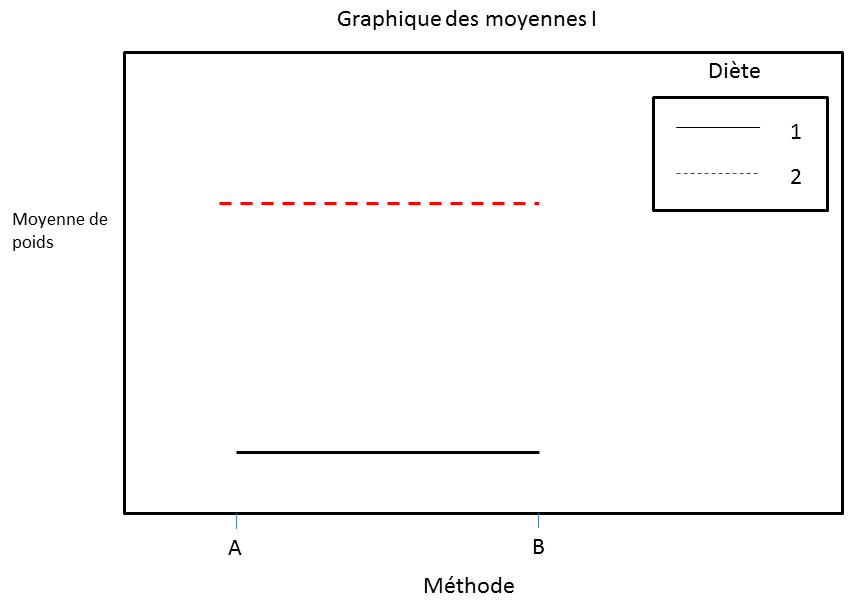
\includegraphics[width=0.45\textwidth]{fig/moy1}\hfill
  
\includegraphics[width=0.45\textwidth]{fig/moy2}\\[4pt]
  
\includegraphics[width=0.45\textwidth]{fig/moy3}\hfill
  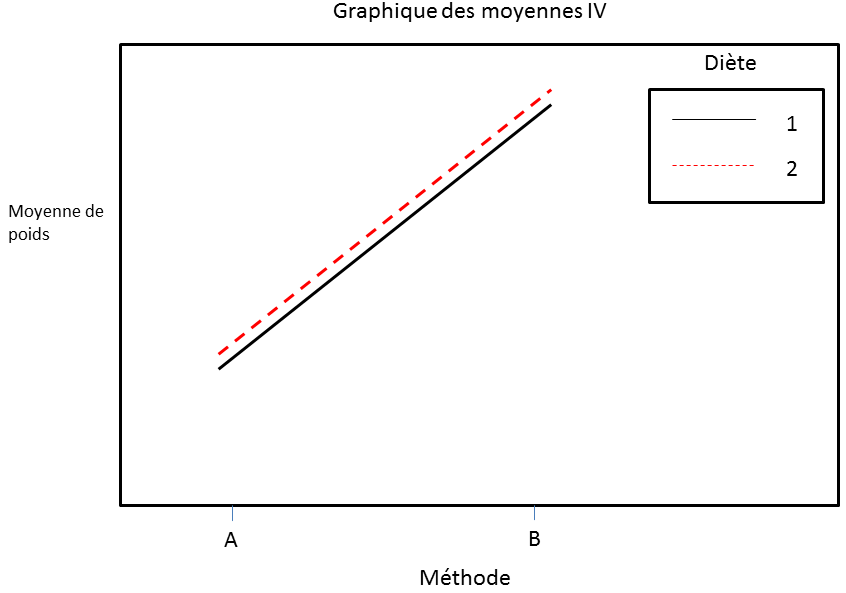
\includegraphics[width=0.45\textwidth]{fig/moy4}\\[4pt]
  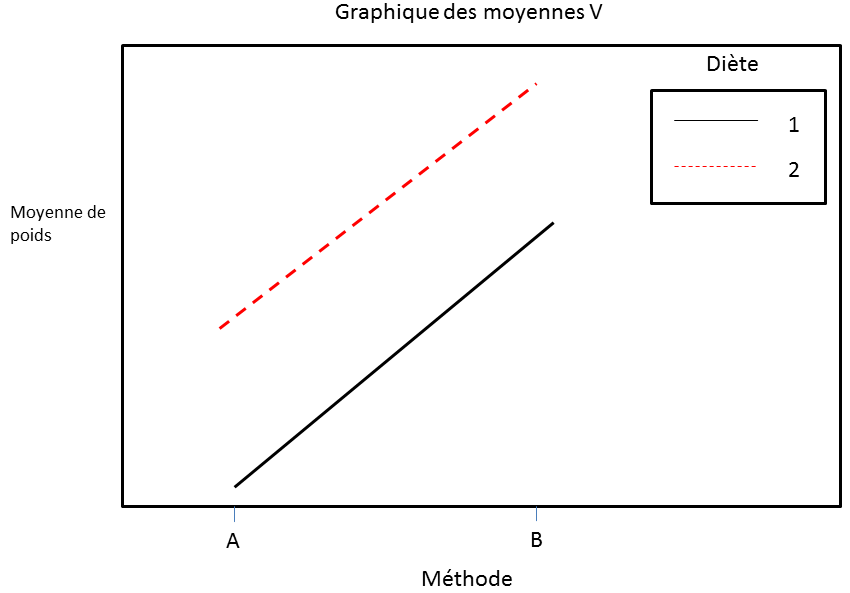
\includegraphics[width=0.45\textwidth]{fig/moy5}
\end{center}
\begin{solution}
\begin{enumerate}[label=(\roman*)]
  \item Graphique II, aucun effet.
  \item Graphique IV, effet méthode.
  \item Graphique I, effet diète.
  \item Graphique V, effet diète et effet méthode.
  \item Graphique III, interaction : diète et méthode ont un effet, qui dépend du niveau de
  l'autre facteur.
\end{enumerate}
\end{solution}
\end{exercice}

\begin{exercice}
Vous effectuez une expérience à un facteur et voulez vous assurer que les postulats émis sur
les termes d'erreur sont raisonnablement respectés. Déterminez lequel/lesquels des
graphiques correspond(ent) à chaque énoncé.
\begin{enumerate}[label=(\alph*)]
  \item La variance des termes d'erreur n'est pas homogène :
  \item La variance des termes d'erreur est homogène :
  \item La normalité des termes d'erreur est respectée :
  \item Les termes d'erreur ne suivent pas une loi normale :
\end{enumerate}
\begin{center}
  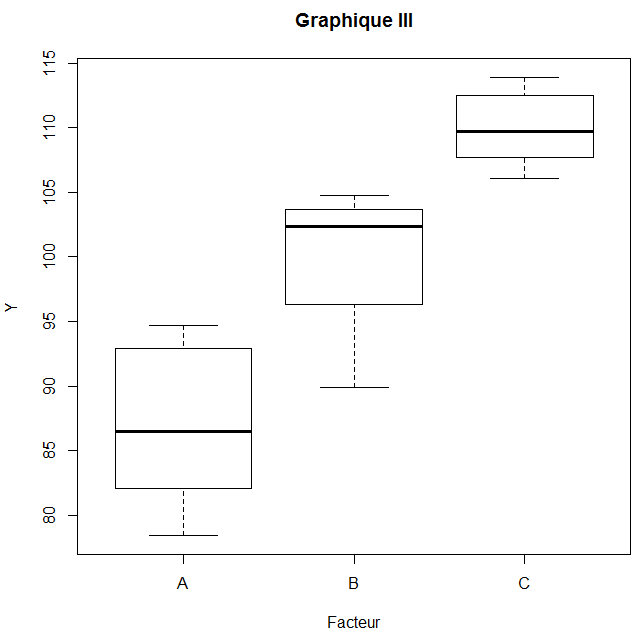
\includegraphics[width=0.42\textwidth]{fig/anovadiag1}\hfill
  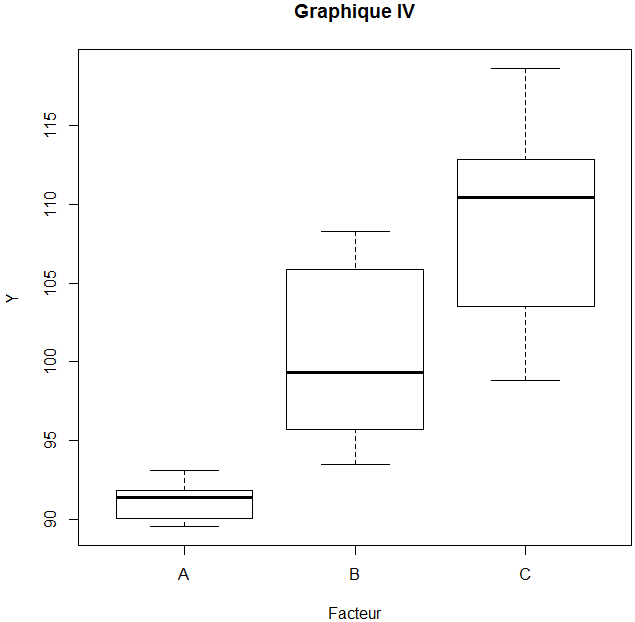
\includegraphics[width=0.42\textwidth]{fig/anovadiag2}\\[4pt]
  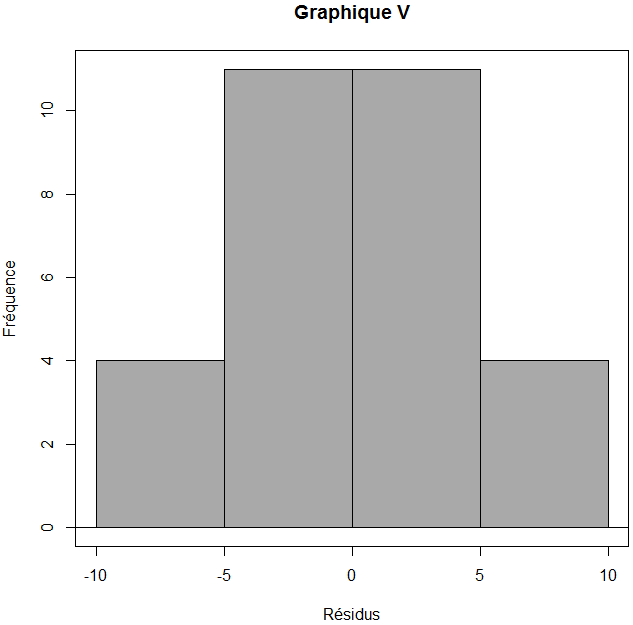
\includegraphics[width=0.42\textwidth]{fig/anovadiag3}\hfill
  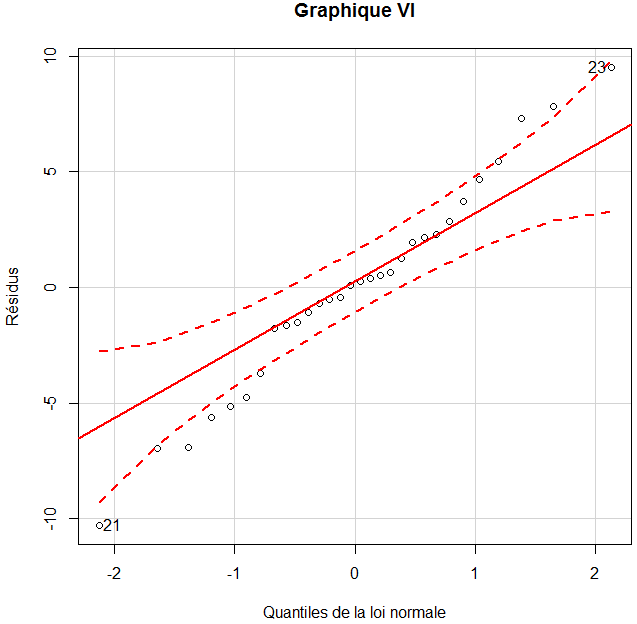
\includegraphics[width=0.42\textwidth]{fig/anovadiag4}\\[4pt]
  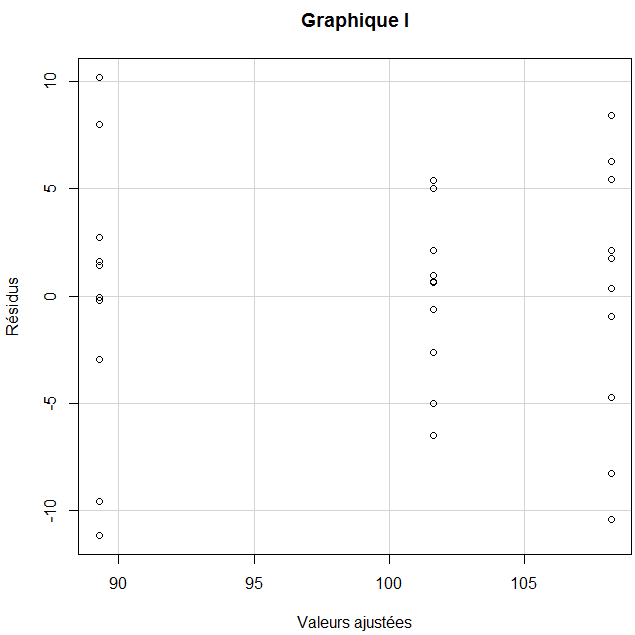
\includegraphics[width=0.42\textwidth]{fig/anovadiag5}\hfill
  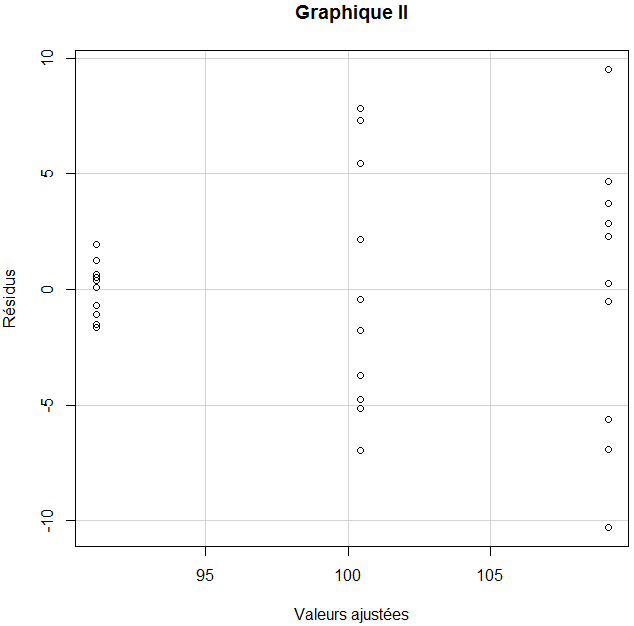
\includegraphics[width=0.42\textwidth]{fig/anovadiag6}
\end{center}
\begin{solution}
\begin{enumerate}[label=(\alph*)]
  \item Les graphiques II et IV.
  \item Le graphique I.
  \item Le graphique V (cloche symétrique unimodale).
  \item Le graphique VI (plusieurs points sortent des limites pointillées, pas de ligne
  droite).
\end{enumerate}
\end{solution}
\end{exercice}

\begin{exercice}
Déterminez si les énoncés suivants sont vrais ou faux.
\begin{enumerate}[label=(\alph*)]
  \item Dans un modèle d'analyse de la variance à un facteur, le paramètre $\sigma^2$
  représente la variance des $Y_{ij}$ autour de la moyenne globale $\mu$.
  \item Dans un plan à blocs aléatoires, on considère que les observations d'un même bloc
  sont dépendantes, et que les observations de blocs différents sont indépendantes.
  \item On pige $n=5$ observations dans chacune des 3 populations suivantes :
  $N(12,3)$, $N(15,3)$, $N(18,3)$. On calcule la statistique $F_1$ de la table d'anova.
  On pige $n=5$ observations dans chacune des 3 populations suivantes :
  $N(12,15)$, $N(15,15)$, $N(18,15)$. On calcule la statistique $F_2$ de la table d'anova.
  La valeur de $F_1$ aura tendance à être plus faible que $F_2$.
  \item Dans un modèle d'analyse de la variance à deux facteurs, si on obtient la table
  d'anova suivante, on conclura que seul le facteur A a un effet sur la valeur de $Y$.
\begin{verbatim}
Anova Table (Type II tests)
Response: Reponse
                  Sum Sq  Df  F value    Pr(>F)
FacteurA          100.33   2    7.525  0.004216 **
FacteurB           13.50   1    2.025  0.171830
FacteurA:FacteurB 688.00   2   51.600 3.515e-08 ***
Residuals         120.00  18
\end{verbatim}
  \item L'analyse de variance précédente a été faite à partir de 19 observations.
\end{enumerate}
\begin{solution}
\begin{enumerate}[label=(\alph*)]
  \item \textbf{Faux.} C'est la variance des $Y_{ij}$ autour de la moyenne locale de chaque
  traitement $\mu_i$.
  \item \textbf{Vrai.}
  \item \textbf{Faux.} La variance intra-traitements ($\sigma^2$) est plus élevée dans le
  2\ieme{} cas. Ainsi, le $MSE$ sera probablement plus grand dans le 2\ieme{} cas, tandis
  que le $MS_{trt}$ devrait être similaire dans les 2 cas (car les moyennes théoriques sont
  égales). Donc $F_2$ aura tendance à être inférieur.
  \item \textbf{Faux.} Si l'interaction est significative, on n'interprète pas les tests F
  sur les facteurs individuels. On peut conclure que les deux facteurs ont un effet, mais ce
  dernier n'est pas le même selon le niveau de l'autre facteur.
  \item \textbf{Faux.} $abn=24$.
\end{enumerate}
\end{solution}
\end{exercice}

\chapitre{10}{Régression linéaire simple}

\begin{exercice}
Pour estimer les stocks excédentaires de l'année courante, une entreprise fabriquant des
pneus a tiré au hasard 6 détaillants chez qui elle vend ses produits ; ceux-ci ont fourni
les chiffres de l'inventaire de l'année passée à pareille date ($X$) et l'inventaire actuel
($Y$) reproduits dans le tableau suivant :
\begin{center}
\begin{tabular}{l*{6}{c}}
  \toprule
  $X$ & 70 & 260 & 150 & 100 & 20 & 60\\
  $Y$ & 60 & 320 & 230 & 120 & 50 & 60\\
  \bottomrule
\end{tabular}
\end{center}
On donne les sommes suivantes :
\[
  \sum_{i=1}^{6}x_i=660,\quad \sum_{i=1}^{6}y_i=840,\quad
  \sum_{i=1}^{6}x_i^2=109\,000,\quad \sum_{i=1}^{6}y_i^2=179\,400,\quad
  \sum_{i=1}^{6}x_iy_i=138\,500.
\]
\begin{enumerate}[label=(\alph*)]
  \item Trouver l'équation de la droite de régression et interpréter la valeur de
  $\hat\beta_1$ dans le contexte de ce problème.
  \item Construire la table d'analyse de la variance.
  \item Déterminer s'il existe une relation linéaire significative entre les inventaires de
  cette année et de l'année passée au seuil $\alpha=5\,\%$.
  \item Calculer la proportion de variabilité de l'inventaire de cette année expliquée par
  celui de l'année passée.
\end{enumerate}
\begin{solution}
\begin{enumerate}[label=(\alph*)]
  \item On calcule
  \[
    S_{XX}=\sum x_i^2-\frac{\left(\sum x_i\right)^2}{n}=109\,000-\frac{660^2}{6}=36\,400,
  \]
  $\bar x=660/6=110$, $\bar y=840/6=140$,
  \[
    S_{XY}=\sum x_iy_i-\frac{\sum x_i\sum y_j}{n}=138\,500-\frac{660\times 840}{6}=46\,100.
  \]
  Donc $\hat\beta_1=\frac{S_{XY}}{S_{XX}}=\frac{46\,100}{36\,400}=1,266$ et
  $\hat\beta_0=\bar y-\hat\beta_1\bar x=140-1,266(110)=0,7$.

  Interprétations : $\hat\beta_0=0,7$ : s'il y a 0 pneu l'année précédente, on espère en
  moyenne 0,7 pneu cette année. $\hat\beta_1=1,266$ : si le nombre de pneus l'année
  précédente augmente de 1 pneu, l'inventaire espéré pour l'année courante augmente de
  1,266 pneu.
  \item
  \[
    SST=S_{YY}=\sum y_i^2-\frac{\left(\sum y_i\right)^2}{n}=179\,400-\frac{840^2}{6}=61\,800,
  \]
  \[
    SSR=\frac{S_{XY}^2}{S_{XX}}=\hat\beta_1S_{XY}=1,266(46\,100)=58\,363,
  \]
  donc $SSE=SST-SSR=61\,800-58\,363=3\,437$.
  \begin{center}
  \begin{tabular}{lcccc}
    \toprule
    Source & SS & d.l. & CM & $F$\\
    \midrule
    Régression & 58\,363 & 1 & $58\,363$ & $\frac{58\,363}{859,4}=67,9$\\[3pt]
    Erreur & 3\,437 & $6-2=4$ & $3\,437/4=859,4$ & \\[3pt]
    Total & 61\,800 & $6-1=5$ & & \\
    \bottomrule
  \end{tabular}
  \end{center}
  \item On teste $H_0:\beta_1=0$ contre $H_1:\beta_1\neq 0$. On a $F_{0,05;1;4}=7,71$.
  Comme $67,9>7,71$, on rejette $H_0$ et donc oui, il y a une relation significative.
  \item On nous demande $R^2=\frac{SSR}{SST}=\frac{58\,363}{61\,800}=94,4\,\%$.
\end{enumerate}
\end{solution}
\end{exercice}

\begin{exercice}
On a ajusté un modèle de régression linéaire simple pour le prix de vente d'une maison (en
milliers de \$) en fonction de l'évaluation de cette maison (en milliers de \$) à l'aide
d'un jeu de données de 25 observations. On a obtenu les valeurs suivantes :
\[
  \hat\beta_0=20,94\qquad \hat\beta_1=1,07\qquad \hat\sigma^2=MSE=1075.
\]
De plus, on vous indique que $\bar x=201,75$ et $S_{xx}=5\,209\,571$.
\begin{enumerate}[label=(\alph*)]
  \item Quel est le prix de vente moyen pour les maisons évaluées à 200~000~\$ ?
  \item Un ami vient de mettre sa maison en vente, évaluée à 280~000~\$. Construisez un
  intervalle à 95\,\% pour le prix de vente de sa maison.
  \item On veut maintenant vérifier la validité des postulats du modèle de régression. Parmi
  les graphiques ci-dessous, lequel permet de valider le postulat de normalité des erreurs ?
  Qu'en déduisez-vous ?
  \begin{center}
    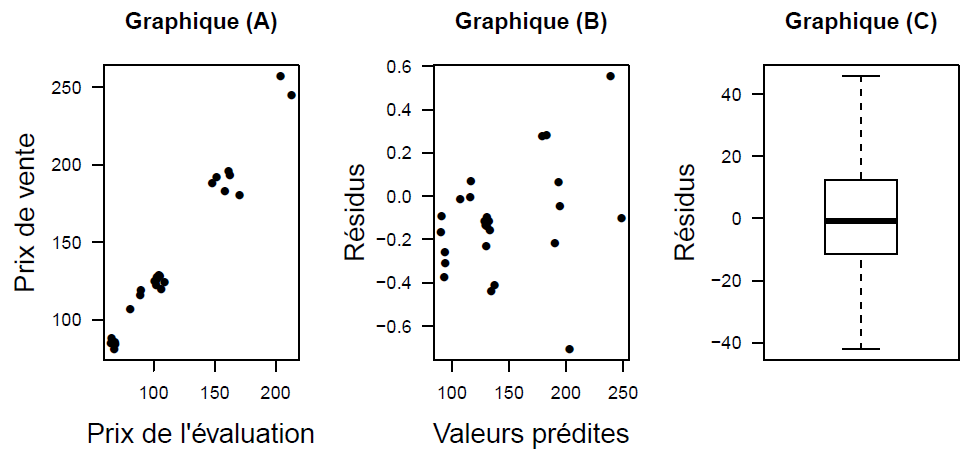
\includegraphics[width=0.95\textwidth]{fig/rls_graphs}
  \end{center}
\end{enumerate}
\begin{solution}
\begin{enumerate}[label=(\alph*)]
  \item On veut une estimation de $E(Y\,|\,X=200)=\beta_0+\beta_1(200)$. Donc,
  \[
    \hat\beta_0+\hat\beta_1(200)=20,94+1,07(200)=234,94\ \text{milliers de \$}.
  \]
  \item On veut un intervalle de confiance pour \emph{une seule} observation (intervalle de
  prévision), quand $X=280$ :
  \begin{align*}
    &\hat\beta_0+\hat\beta_1(280)\pm t_{\alpha/2;n-2}
    \sqrt{MSE\left(1+\frac1n+\frac{(\bar x-280)^2}{S_{XX}}\right)}\\
    &\quad=20,94+1,07(280)\pm t_{0,025;23}
    \sqrt{1075\left(1+\frac{1}{25}+\frac{(201,75-280)^2}{5\,209\,571}\right)}\\
    &\quad=320,54\pm 69,22=(251,31\,;\;389,76)\ \text{milliers de \$},
  \end{align*}
  avec $t_{0,025;23}=2,069$.
  \item C'est le graphique (C) (diagramme en boîte des résidus) qui permet de valider le
  postulat de normalité des erreurs. Ici, il est très symétrique et n'a aucune valeur
  extrême, donc le postulat est respecté.

  À titre indicatif : le graphique (A) ($Y$ versus $X$) permet de valider la linéarité de la
  relation, bien respectée ici ; le graphique (B) (résidus versus valeurs ajustées) permet
  de valider l'homogénéité de la variance — ici, un entonnoir se dessine, il y aurait lieu
  d'essayer quelques transformations de la variable $Y$.
\end{enumerate}
\end{solution}
\end{exercice}

\begin{exercice}
Vous effectuez une analyse de régression et voulez vous assurer que les postulats émis sur
les termes d'erreur sont raisonnables. Déterminez lequel/lesquels des graphiques
correspond(ent) à chaque énoncé. S'il s'agit d'un problème avec l'un des postulats, suggérez
une solution.
\begin{enumerate}[label=(\alph*)]
  \item La linéarité de la relation $X$-$Y$ est respectée :
  \item La linéarité de la relation $X$-$Y$ n'est pas respectée :
  \item Il y a homoscédasticité :
  \item Il y a hétéroscédasticité :
  \item La normalité des erreurs est respectée :
  \item La normalité des erreurs n'est pas respectée :
\end{enumerate}
\begin{center}
  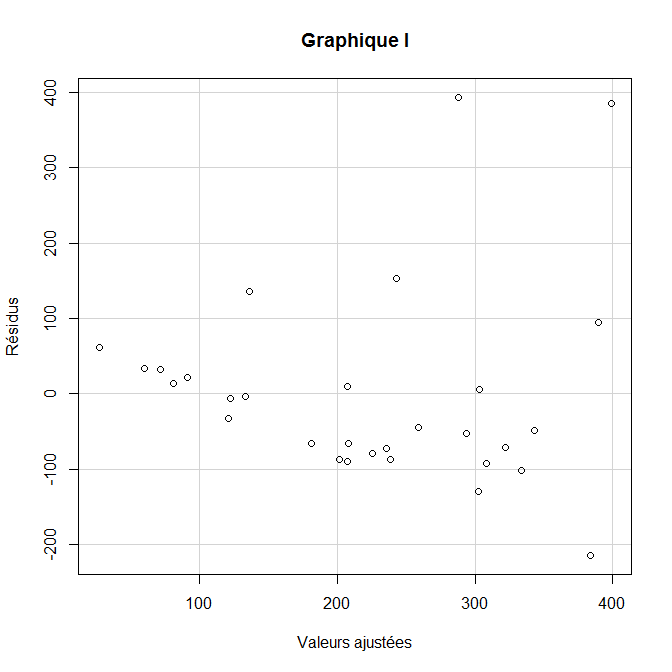
\includegraphics[width=0.42\textwidth]{fig/regdiag1}\hfill
  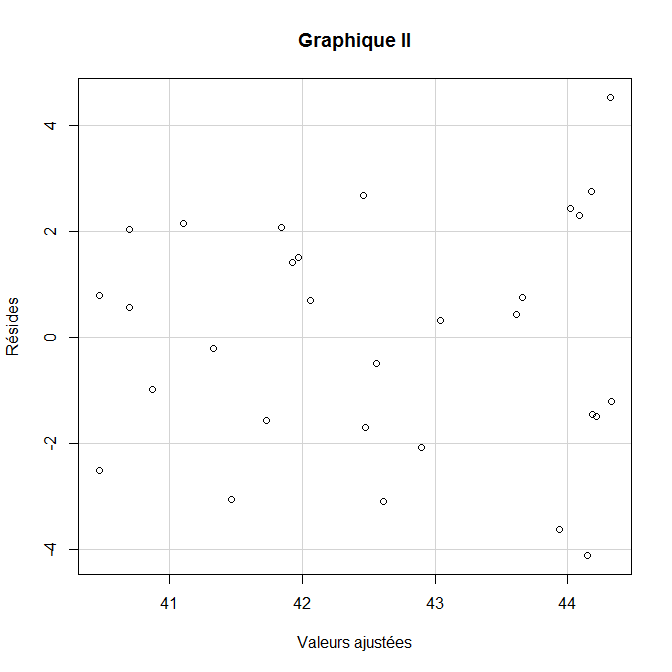
\includegraphics[width=0.42\textwidth]{fig/regdiag2}\\[4pt]
  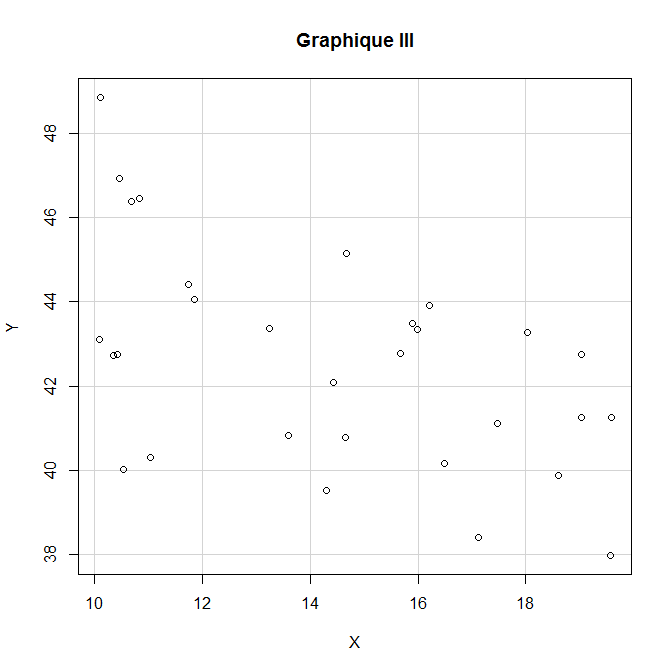
\includegraphics[width=0.42\textwidth]{fig/regdiag3}\hfill
  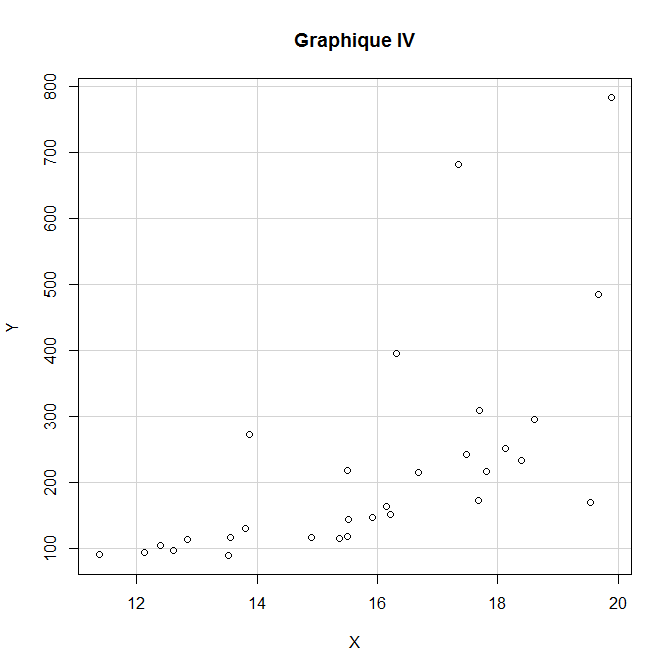
\includegraphics[width=0.42\textwidth]{fig/regdiag4}\\[4pt]
  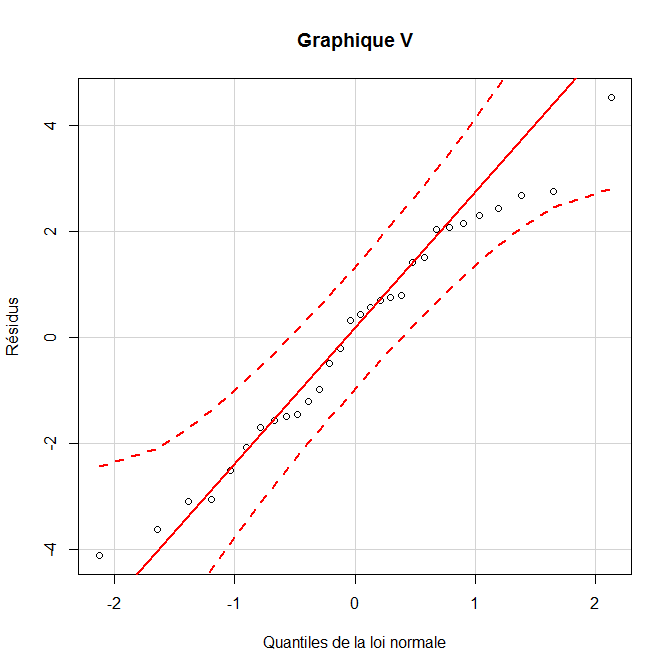
\includegraphics[width=0.42\textwidth]{fig/regdiag5}\hfill
  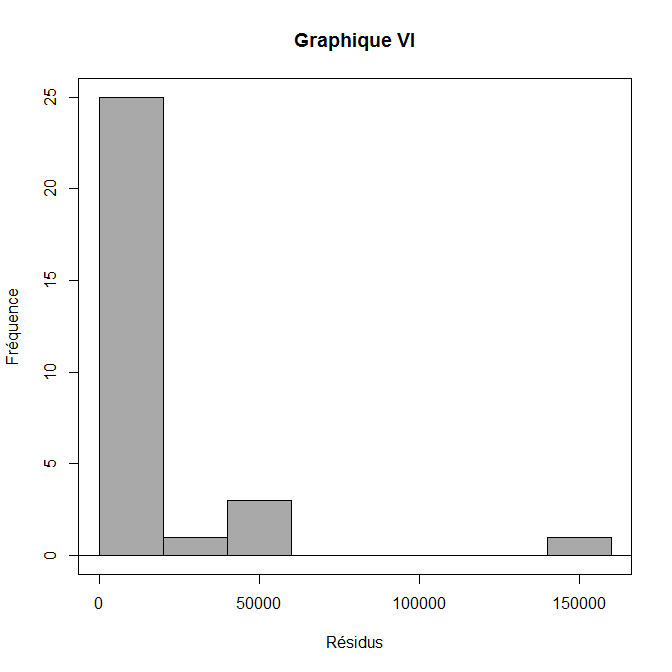
\includegraphics[width=0.42\textwidth]{fig/regdiag6}
\end{center}
\begin{solution}
\begin{enumerate}[label=(\alph*)]
  \item Les graphiques II et III.
  \item Le graphique IV. Solution : ajuster un modèle quadratique ou transformer $Y$.
  \item Les graphiques II et III.
  \item Les graphiques I et IV. Solution : transformer $Y$ ($\sqrt Y$, $\ln Y$,
  $1/\sqrt Y$, $1/Y$, etc.).
  \item Le graphique V.
  \item Le graphique VI. Solution : transformer $Y$ ou retirer la valeur extrême pour
  l'inférence.
\end{enumerate}
\end{solution}
\end{exercice}

\begin{exercice}
Déterminez si les énoncés suivants sont vrais ou faux.
\begin{enumerate}[label=(\alph*)]
  \item Si tous les points $(x_1,y_1),\dots,(x_9,y_9)$ sont parfaitement alignés selon une
  droite de pente positive, alors on sait que $\hat\beta_1=1$, $SSE=0$ et $r=1$.
  \item Supposons que le modèle $Y\sim N(\beta_0+\beta_1X,\sigma^2)$ décrit bien la relation
  entre $Y$ et $X$. Alors les prédictions de $Y$ pour $X=x_0$ seront plus précises si on
  choisit des $x_i$ très dispersés, une grande taille d'échantillon, et une valeur $x_0$
  assez proche de $\bar x$.
\end{enumerate}
\begin{solution}
\begin{enumerate}[label=(\alph*)]
  \item \textbf{Faux.} L'estimation de $\beta_1$ sera positive, mais pas nécessairement
  égale à 1.
  \item \textbf{Vrai.}
\end{enumerate}
\end{solution}
\end{exercice}

\chapitre{11}{Régression linéaire multiple}

\begin{exercice}
On cherche à construire un modèle pour expliquer et prédire $Y$, la consommation
d'électricité (en kWh), des maisons unifamiliales d'une région. Les variables explicatives
disponibles sont $X_1$, le nombre d'habitants ; $X_2$, la superficie habitable (en milliers
de pieds carrés) ; $X_3$, le revenu annuel du ménage (en milliers de dollars) et $X_4$, le
montant annuel de la taxe foncière (en milliers de dollars).

On recueille des données pour 25 maisons unifamiliales de cette région et on ajuste un
modèle de régression linéaire multiple à nos observations. Après vérification, les postulats
du modèle semblent raisonnablement respectés. Un extrait de la sortie R Commander obtenue
est donné ci-dessous.
\begin{verbatim}
> summary(RegModel.2)
Coefficients:
            Estimate Std. Error
(Intercept) 57.80968    9.92327
X1           6.61733    0.95758
X2          28.46419    8.40441
X3           0.05516    0.14109
X4           4.48517    8.30631
---
Residual standard error: 4.378 on 20 degrees of freedom
Multiple R-squared: 0.9072,    Adjusted R-squared: 0.8886
F-statistic: 48.88 on 4 and 20 DF,  p-value: 4.773e-10
\end{verbatim}
\begin{enumerate}[label=(\alph*)]
  \item Peut-on conclure qu'au moins une des quatre variables explicatives est
  significative, au seuil de 5\,\% ?
  \item Donnez une estimation ponctuelle et un intervalle de confiance à 95\,\% pour l'effet
  d'une hausse de la superficie habitable de 1 millier de pieds carrés sur la consommation
  d'électricité espérée, toute autre variable explicative restant inchangée.
  \item Le graphique ci-dessous permet de sélectionner le meilleur sous-modèle selon le
  critère du $R^2_{ajust\acute e}$ produit par R Commander. Selon ce graphique, quelles
  variables explicatives sont retenues dans le meilleur sous-modèle selon le critère
  $R^2_{ajust\acute e}$ ?
  \begin{center}
    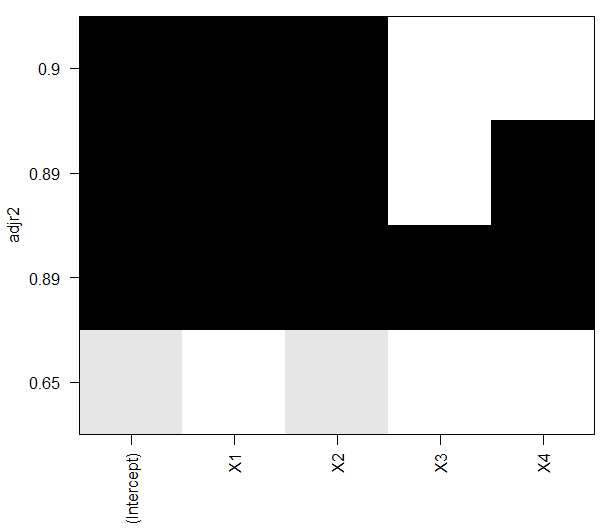
\includegraphics[width=0.55\textwidth]{fig/adjr2}
  \end{center}
\end{enumerate}
\begin{solution}
\begin{enumerate}[label=(\alph*)]
  \item Le test F sur l'importance globale de la régression oppose
  \[
    H_0:\beta_1=\beta_2=\beta_3=\beta_4=0
    \quad\text{à}\quad
    H_1:\text{au moins un }\beta_j\neq 0\text{ pour }j=1,2,3,4.
  \]
  Puisque $\alpha^*=4,77\times 10^{-10}<0,05$, on rejette $H_0$. Ainsi, au moins une des 4
  variables est liée linéairement à la consommation d'électricité.
  \item La hausse moyenne de $Y$ lorsque $X_2$ augmente de 1 est $\beta_2$ :
  \begin{align*}
    IC(\beta_2)&=\hat\beta_2\pm t_{\alpha/2;n-k-1}\times\text{erreur-type}(\hat\beta_2)\\
    &=28,46419\pm 2,086\times(8,40441)
    =28,46419\pm 17,53160
    =[10,933\,;\;45,996].
  \end{align*}
  \item Les carrés noirs et gris sur une même ligne indiquent les variables retenues dans un
  modèle. Puisqu'on cherche à maximiser le $R^2_{ajust\acute e}$, le meilleur modèle selon
  ce critère est celui de la ligne du haut, c'est-à-dire celui incluant seulement
  $X_1$ (nombre d'habitants) et $X_2$ (superficie habitable) :
  \[
    Y_i=\beta_0+\beta_1X_{1i}+\beta_2X_{2i}+E_i.
  \]
  \emph{Note :} les coefficients auraient de nouvelles estimations si on ajustait le modèle
  réduit dans R Commander sur les mêmes données.
\end{enumerate}
\end{solution}
\end{exercice}

\begin{exercice}
Une étude est menée dans l'espoir de trouver la bonne quantité d'un catalyseur à ajouter à
un procédé afin de maximiser la qualité du produit obtenu. On répète une expérience 20 fois
et on obtient les résultats suivants :
\begin{itemize}
  \item $Y_i$, un indice de qualité du produit final lors de l'expérience $i$ (plus $Y_i$
  est élevé, meilleur est le produit),
  \item $C_i$, la quantité de catalyseur utilisée lors de l'expérience $i$ et
  \item $P_i$, la quantité de pétrole utilisée dans l'expérience $i$.
\end{itemize}
Après discussion avec vos collègues et une revue de la littérature, vous ajustez le modèle
de régression linéaire multiple ci-dessous à vos données, pour lequel les 4 postulats usuels
s'avèrent raisonnables :
\[
  Y_i=\beta_0+\beta_1X_{i1}+\beta_2X_{i2}+\beta_3X_{i3}+E_i,\qquad i=1,\dots,20,
\]
où $X_{i1}=C_i$, $X_{i2}=C_i^2$, $X_{i3}=P_i$ et les $E_i$ sont des termes d'erreur i.i.d.
$N(0,\sigma^2)$. Voici la sortie R Commander, où quelques valeurs sont remplacées par
AAAAA, BBBBB, etc.
\begin{verbatim}
lm(formula = Y ~ X1 + X2 + X3, data = Qualite)
Residuals:
    Min      1Q  Median      3Q     Max
-7.5562 -2.7782  0.1606  4.1300  6.6078
Coefficients:
             Estimate Std. Error t value Pr(>|t|)
(Intercept) 113.13496   38.09154   2.970  0.00903 **
X1            8.86398    3.15453   2.810  0.01258 *
X2           -0.17704    0.06996  -2.531  0.02226 *
X3            9.99053    0.48986  20.395 7.08e-13 ***
---
Residual standard error: 4.612 on 16 degrees of freedom
Multiple R-squared: AAAAA,    Adjusted R-squared: BBBBB
F-statistic: CCCCC on DDDDD and EEEEE DF,  p-value: 3.415e-12
\end{verbatim}
\begin{enumerate}[label=(\alph*)]
  \item Donnez une estimation de la quantité de catalyseur qui maximise l'indice de qualité
  espéré, lorsque la quantité de pétrole est égale à 3 unités.
  \item Avant l'expérience, un de vos collègues avait dit qu'une hausse d'une unité de la
  quantité de pétrole hausserait l'indice de qualité espéré d'au moins 9 unités. Les données
  supportent-elles l'hypothèse de votre collègue au seuil de 5\,\% ?
  \item Sachant que $SST=10\,701,3$, trouvez les valeurs manquantes AAAAA, BBBBB, etc.
  \item Le tableau ci-dessous donne la liste de tous les sous-modèles possibles (chacun
  incluant une ordonnée à l'origine), ainsi que leur $R^2_{ajust\acute e}$. Quel est le
  meilleur modèle selon ce critère ?
  \begin{center}
  \begin{tabular}{l*{7}{c}}
    \toprule
    Sous-modèle & $X_1,X_2,X_3$ & $X_1,X_2$ & $X_1,X_3$ & $X_2,X_3$ & $X_1$ & $X_2$ & $X_3$\\
    \midrule
    $R^2_{ajust\acute e}$ & 0,962 & 0,041 & 0,955 & 0,950 & 0,0001 & 0,005 & 0,920\\
    \bottomrule
  \end{tabular}
  \end{center}
\end{enumerate}
\begin{solution}
\begin{enumerate}[label=(\alph*)]
  \item On a
  \[
    E(Y_i\,|\,X)=\beta_0+\beta_1c_i+\beta_2c_i^2+\beta_3P_i.
  \]
  Lorsque $P_i=3$, il s'agit d'une parabole :
  $E(Y_i\,|\,X)=[\beta_0+3\beta_3]+\beta_1c_i+\beta_2c_i^2$, ouverte vers le bas si
  $\beta_2<0$. On cherche la valeur $c_0$ qui maximise $E(Y_i\,|\,X)$ :
  \[
    \frac{\partial E(Y_i\,|\,X)}{\partial c}=\beta_1+2\beta_2c=0
    \;\Longrightarrow\;c_0=\frac{-\beta_1}{2\beta_2},
  \]
  et la valeur estimée de $c_0$ est
  \[
    \hat c_0=\frac{-\hat\beta_1}{2\hat\beta_2}=\frac{-8,86398}{2(-0,17704)}=25,03.
  \]
  \item On veut tester $H_0:\beta_3=9$ contre $H_1:\beta_3>9$.
  On rejettera $H_0$ si $t_0=\frac{\hat\beta_3-9}{se(\hat\beta_3)}>t_{0,05;16}=1,746$.
  Calcul de la statistique observée :
  \[
    t_{obs}=\frac{\hat\beta_3-\beta_{3,0}}{se(\hat\beta_3)}
    =\frac{9,99053-9}{0,48986}=2,022.
  \]
  Puisque $2,022>1,746$, on rejette $H_0$. L'hypothèse du collègue est supportée par les
  données : une hausse de 1 unité de pétrole augmente en moyenne d'au moins 9 unités
  l'indice de qualité, si $\alpha=0,05$ et que la quantité de catalyseur $c_i$ reste
  inchangée.
  \item On sait que DDDDD~$=3$ et que EEEEE~$=16$. On a $MSE=4,612^2$, donc
  $\frac{SSE}{16}=4,612^2$ et $SSE=340,3$. Ainsi,
  \[
    SSR=SST-SSE=10\,701,3-340,3=10\,361
    \qquad\text{et}\qquad
    \text{AAAAA}=R^2=\frac{10\,361}{10\,701,3}=0,968.
  \]
  \[
    \text{BBBBB}=R^2_{ajust\acute e}=1-\frac{SSE/(n-k-1)}{SST/(n-1)}
    =1-\frac{340,3/(20-3-1)}{10\,701,3/(20-1)}=0,962.
  \]
  \[
    \text{CCCCC}=F_0=\frac{SSR/k}{SSE/(n-k-1)}=\frac{10\,361/3}{340,3/16}=162,4.
  \]
  \item On cherche le modèle avec le $R^2_{ajust\acute e}$ \emph{le plus élevé}, donc on
  choisit le modèle complet $Y_i=\beta_0+\beta_1x_{i1}+\beta_2x_{i2}+\beta_3x_{i3}+E_i$.
\end{enumerate}
\end{solution}
\end{exercice}

\begin{exercice}
Déterminez si les énoncés suivants sont vrais ou faux.
\begin{enumerate}[label=(\alph*)]
  \item Le meilleur modèle de régression à 3 variables explicatives est celui comprenant les
  3 variables les plus corrélées avec la variable réponse $Y$.
  \item Plus on ajoute de variables explicatives à un modèle de régression, plus la valeur
  de $SSE$ diminue.
\end{enumerate}
\begin{solution}
\begin{enumerate}[label=(\alph*)]
  \item \textbf{Faux.} C'est vrai pour une variable explicative, mais pas pour plusieurs.
  S'il y a multicolinéarité ($X_i$ corrélées), les variables explicatives sont redondantes
  et pourraient ne pas être nécessaires ensemble, dans un même modèle pour prédire $Y$.
  \item \textbf{Vrai.}
\end{enumerate}
\end{solution}
\end{exercice}
